
\documentclass{article} % For LaTeX2e
\usepackage{iclr2021_conference,times}

% Optional math commands from https://github.com/goodfeli/dlbook_notation.
%%%%% NEW MATH DEFINITIONS %%%%%

\usepackage{amsmath,amsfonts,bm}

% Mark sections of captions for referring to divisions of figures
\newcommand{\figleft}{{\em (Left)}}
\newcommand{\figcenter}{{\em (Center)}}
\newcommand{\figright}{{\em (Right)}}
\newcommand{\figtop}{{\em (Top)}}
\newcommand{\figbottom}{{\em (Bottom)}}
\newcommand{\captiona}{{\em (a)}}
\newcommand{\captionb}{{\em (b)}}
\newcommand{\captionc}{{\em (c)}}
\newcommand{\captiond}{{\em (d)}}

% Highlight a newly defined term
\newcommand{\newterm}[1]{{\bf #1}}


% Figure reference, lower-case.
\def\figref#1{figure~\ref{#1}}
% Figure reference, capital. For start of sentence
\def\Figref#1{Figure~\ref{#1}}
\def\twofigref#1#2{figures \ref{#1} and \ref{#2}}
\def\quadfigref#1#2#3#4{figures \ref{#1}, \ref{#2}, \ref{#3} and \ref{#4}}
% Section reference, lower-case.
\def\secref#1{section~\ref{#1}}
% Section reference, capital.
\def\Secref#1{Section~\ref{#1}}
% Reference to two sections.
\def\twosecrefs#1#2{sections \ref{#1} and \ref{#2}}
% Reference to three sections.
\def\secrefs#1#2#3{sections \ref{#1}, \ref{#2} and \ref{#3}}
% Reference to an equation, lower-case.
\def\eqref#1{equation~\ref{#1}}
% Reference to an equation, upper case
\def\Eqref#1{Equation~\ref{#1}}
% A raw reference to an equation---avoid using if possible
\def\plaineqref#1{\ref{#1}}
% Reference to a chapter, lower-case.
\def\chapref#1{chapter~\ref{#1}}
% Reference to an equation, upper case.
\def\Chapref#1{Chapter~\ref{#1}}
% Reference to a range of chapters
\def\rangechapref#1#2{chapters\ref{#1}--\ref{#2}}
% Reference to an algorithm, lower-case.
\def\algref#1{algorithm~\ref{#1}}
% Reference to an algorithm, upper case.
\def\Algref#1{Algorithm~\ref{#1}}
\def\twoalgref#1#2{algorithms \ref{#1} and \ref{#2}}
\def\Twoalgref#1#2{Algorithms \ref{#1} and \ref{#2}}
% Reference to a part, lower case
\def\partref#1{part~\ref{#1}}
% Reference to a part, upper case
\def\Partref#1{Part~\ref{#1}}
\def\twopartref#1#2{parts \ref{#1} and \ref{#2}}

\def\ceil#1{\lceil #1 \rceil}
\def\floor#1{\lfloor #1 \rfloor}
\def\1{\bm{1}}
\newcommand{\train}{\mathcal{D}}
\newcommand{\valid}{\mathcal{D_{\mathrm{valid}}}}
\newcommand{\test}{\mathcal{D_{\mathrm{test}}}}

\def\eps{{\epsilon}}


% Random variables
\def\reta{{\textnormal{$\eta$}}}
\def\ra{{\textnormal{a}}}
\def\rb{{\textnormal{b}}}
\def\rc{{\textnormal{c}}}
\def\rd{{\textnormal{d}}}
\def\re{{\textnormal{e}}}
\def\rf{{\textnormal{f}}}
\def\rg{{\textnormal{g}}}
\def\rh{{\textnormal{h}}}
\def\ri{{\textnormal{i}}}
\def\rj{{\textnormal{j}}}
\def\rk{{\textnormal{k}}}
\def\rl{{\textnormal{l}}}
% rm is already a command, just don't name any random variables m
\def\rn{{\textnormal{n}}}
\def\ro{{\textnormal{o}}}
\def\rp{{\textnormal{p}}}
\def\rq{{\textnormal{q}}}
\def\rr{{\textnormal{r}}}
\def\rs{{\textnormal{s}}}
\def\rt{{\textnormal{t}}}
\def\ru{{\textnormal{u}}}
\def\rv{{\textnormal{v}}}
\def\rw{{\textnormal{w}}}
\def\rx{{\textnormal{x}}}
\def\ry{{\textnormal{y}}}
\def\rz{{\textnormal{z}}}

% Random vectors
\def\rvepsilon{{\mathbf{\epsilon}}}
\def\rvtheta{{\mathbf{\theta}}}
\def\rva{{\mathbf{a}}}
\def\rvb{{\mathbf{b}}}
\def\rvc{{\mathbf{c}}}
\def\rvd{{\mathbf{d}}}
\def\rve{{\mathbf{e}}}
\def\rvf{{\mathbf{f}}}
\def\rvg{{\mathbf{g}}}
\def\rvh{{\mathbf{h}}}
\def\rvu{{\mathbf{i}}}
\def\rvj{{\mathbf{j}}}
\def\rvk{{\mathbf{k}}}
\def\rvl{{\mathbf{l}}}
\def\rvm{{\mathbf{m}}}
\def\rvn{{\mathbf{n}}}
\def\rvo{{\mathbf{o}}}
\def\rvp{{\mathbf{p}}}
\def\rvq{{\mathbf{q}}}
\def\rvr{{\mathbf{r}}}
\def\rvs{{\mathbf{s}}}
\def\rvt{{\mathbf{t}}}
\def\rvu{{\mathbf{u}}}
\def\rvv{{\mathbf{v}}}
\def\rvw{{\mathbf{w}}}
\def\rvx{{\mathbf{x}}}
\def\rvy{{\mathbf{y}}}
\def\rvz{{\mathbf{z}}}

% Elements of random vectors
\def\erva{{\textnormal{a}}}
\def\ervb{{\textnormal{b}}}
\def\ervc{{\textnormal{c}}}
\def\ervd{{\textnormal{d}}}
\def\erve{{\textnormal{e}}}
\def\ervf{{\textnormal{f}}}
\def\ervg{{\textnormal{g}}}
\def\ervh{{\textnormal{h}}}
\def\ervi{{\textnormal{i}}}
\def\ervj{{\textnormal{j}}}
\def\ervk{{\textnormal{k}}}
\def\ervl{{\textnormal{l}}}
\def\ervm{{\textnormal{m}}}
\def\ervn{{\textnormal{n}}}
\def\ervo{{\textnormal{o}}}
\def\ervp{{\textnormal{p}}}
\def\ervq{{\textnormal{q}}}
\def\ervr{{\textnormal{r}}}
\def\ervs{{\textnormal{s}}}
\def\ervt{{\textnormal{t}}}
\def\ervu{{\textnormal{u}}}
\def\ervv{{\textnormal{v}}}
\def\ervw{{\textnormal{w}}}
\def\ervx{{\textnormal{x}}}
\def\ervy{{\textnormal{y}}}
\def\ervz{{\textnormal{z}}}

% Random matrices
\def\rmA{{\mathbf{A}}}
\def\rmB{{\mathbf{B}}}
\def\rmC{{\mathbf{C}}}
\def\rmD{{\mathbf{D}}}
\def\rmE{{\mathbf{E}}}
\def\rmF{{\mathbf{F}}}
\def\rmG{{\mathbf{G}}}
\def\rmH{{\mathbf{H}}}
\def\rmI{{\mathbf{I}}}
\def\rmJ{{\mathbf{J}}}
\def\rmK{{\mathbf{K}}}
\def\rmL{{\mathbf{L}}}
\def\rmM{{\mathbf{M}}}
\def\rmN{{\mathbf{N}}}
\def\rmO{{\mathbf{O}}}
\def\rmP{{\mathbf{P}}}
\def\rmQ{{\mathbf{Q}}}
\def\rmR{{\mathbf{R}}}
\def\rmS{{\mathbf{S}}}
\def\rmT{{\mathbf{T}}}
\def\rmU{{\mathbf{U}}}
\def\rmV{{\mathbf{V}}}
\def\rmW{{\mathbf{W}}}
\def\rmX{{\mathbf{X}}}
\def\rmY{{\mathbf{Y}}}
\def\rmZ{{\mathbf{Z}}}

% Elements of random matrices
\def\ermA{{\textnormal{A}}}
\def\ermB{{\textnormal{B}}}
\def\ermC{{\textnormal{C}}}
\def\ermD{{\textnormal{D}}}
\def\ermE{{\textnormal{E}}}
\def\ermF{{\textnormal{F}}}
\def\ermG{{\textnormal{G}}}
\def\ermH{{\textnormal{H}}}
\def\ermI{{\textnormal{I}}}
\def\ermJ{{\textnormal{J}}}
\def\ermK{{\textnormal{K}}}
\def\ermL{{\textnormal{L}}}
\def\ermM{{\textnormal{M}}}
\def\ermN{{\textnormal{N}}}
\def\ermO{{\textnormal{O}}}
\def\ermP{{\textnormal{P}}}
\def\ermQ{{\textnormal{Q}}}
\def\ermR{{\textnormal{R}}}
\def\ermS{{\textnormal{S}}}
\def\ermT{{\textnormal{T}}}
\def\ermU{{\textnormal{U}}}
\def\ermV{{\textnormal{V}}}
\def\ermW{{\textnormal{W}}}
\def\ermX{{\textnormal{X}}}
\def\ermY{{\textnormal{Y}}}
\def\ermZ{{\textnormal{Z}}}

% Vectors
\def\vzero{{\bm{0}}}
\def\vone{{\bm{1}}}
\def\vmu{{\bm{\mu}}}
\def\vtheta{{\bm{\theta}}}
\def\va{{\bm{a}}}
\def\vb{{\bm{b}}}
\def\vc{{\bm{c}}}
\def\vd{{\bm{d}}}
\def\ve{{\bm{e}}}
\def\vf{{\bm{f}}}
\def\vg{{\bm{g}}}
\def\vh{{\bm{h}}}
\def\vi{{\bm{i}}}
\def\vj{{\bm{j}}}
\def\vk{{\bm{k}}}
\def\vl{{\bm{l}}}
\def\vm{{\bm{m}}}
\def\vn{{\bm{n}}}
\def\vo{{\bm{o}}}
\def\vp{{\bm{p}}}
\def\vq{{\bm{q}}}
\def\vr{{\bm{r}}}
\def\vs{{\bm{s}}}
\def\vt{{\bm{t}}}
\def\vu{{\bm{u}}}
\def\vv{{\bm{v}}}
\def\vw{{\bm{w}}}
\def\vx{{\bm{x}}}
\def\vy{{\bm{y}}}
\def\vz{{\bm{z}}}

% Elements of vectors
\def\evalpha{{\alpha}}
\def\evbeta{{\beta}}
\def\evepsilon{{\epsilon}}
\def\evlambda{{\lambda}}
\def\evomega{{\omega}}
\def\evmu{{\mu}}
\def\evpsi{{\psi}}
\def\evsigma{{\sigma}}
\def\evtheta{{\theta}}
\def\eva{{a}}
\def\evb{{b}}
\def\evc{{c}}
\def\evd{{d}}
\def\eve{{e}}
\def\evf{{f}}
\def\evg{{g}}
\def\evh{{h}}
\def\evi{{i}}
\def\evj{{j}}
\def\evk{{k}}
\def\evl{{l}}
\def\evm{{m}}
\def\evn{{n}}
\def\evo{{o}}
\def\evp{{p}}
\def\evq{{q}}
\def\evr{{r}}
\def\evs{{s}}
\def\evt{{t}}
\def\evu{{u}}
\def\evv{{v}}
\def\evw{{w}}
\def\evx{{x}}
\def\evy{{y}}
\def\evz{{z}}

% Matrix
\def\mA{{\bm{A}}}
\def\mB{{\bm{B}}}
\def\mC{{\bm{C}}}
\def\mD{{\bm{D}}}
\def\mE{{\bm{E}}}
\def\mF{{\bm{F}}}
\def\mG{{\bm{G}}}
\def\mH{{\bm{H}}}
\def\mI{{\bm{I}}}
\def\mJ{{\bm{J}}}
\def\mK{{\bm{K}}}
\def\mL{{\bm{L}}}
\def\mM{{\bm{M}}}
\def\mN{{\bm{N}}}
\def\mO{{\bm{O}}}
\def\mP{{\bm{P}}}
\def\mQ{{\bm{Q}}}
\def\mR{{\bm{R}}}
\def\mS{{\bm{S}}}
\def\mT{{\bm{T}}}
\def\mU{{\bm{U}}}
\def\mV{{\bm{V}}}
\def\mW{{\bm{W}}}
\def\mX{{\bm{X}}}
\def\mY{{\bm{Y}}}
\def\mZ{{\bm{Z}}}
\def\mBeta{{\bm{\beta}}}
\def\mPhi{{\bm{\Phi}}}
\def\mLambda{{\bm{\Lambda}}}
\def\mSigma{{\bm{\Sigma}}}

% Tensor
\DeclareMathAlphabet{\mathsfit}{\encodingdefault}{\sfdefault}{m}{sl}
\SetMathAlphabet{\mathsfit}{bold}{\encodingdefault}{\sfdefault}{bx}{n}
\newcommand{\tens}[1]{\bm{\mathsfit{#1}}}
\def\tA{{\tens{A}}}
\def\tB{{\tens{B}}}
\def\tC{{\tens{C}}}
\def\tD{{\tens{D}}}
\def\tE{{\tens{E}}}
\def\tF{{\tens{F}}}
\def\tG{{\tens{G}}}
\def\tH{{\tens{H}}}
\def\tI{{\tens{I}}}
\def\tJ{{\tens{J}}}
\def\tK{{\tens{K}}}
\def\tL{{\tens{L}}}
\def\tM{{\tens{M}}}
\def\tN{{\tens{N}}}
\def\tO{{\tens{O}}}
\def\tP{{\tens{P}}}
\def\tQ{{\tens{Q}}}
\def\tR{{\tens{R}}}
\def\tS{{\tens{S}}}
\def\tT{{\tens{T}}}
\def\tU{{\tens{U}}}
\def\tV{{\tens{V}}}
\def\tW{{\tens{W}}}
\def\tX{{\tens{X}}}
\def\tY{{\tens{Y}}}
\def\tZ{{\tens{Z}}}


% Graph
\def\gA{{\mathcal{A}}}
\def\gB{{\mathcal{B}}}
\def\gC{{\mathcal{C}}}
\def\gD{{\mathcal{D}}}
\def\gE{{\mathcal{E}}}
\def\gF{{\mathcal{F}}}
\def\gG{{\mathcal{G}}}
\def\gH{{\mathcal{H}}}
\def\gI{{\mathcal{I}}}
\def\gJ{{\mathcal{J}}}
\def\gK{{\mathcal{K}}}
\def\gL{{\mathcal{L}}}
\def\gM{{\mathcal{M}}}
\def\gN{{\mathcal{N}}}
\def\gO{{\mathcal{O}}}
\def\gP{{\mathcal{P}}}
\def\gQ{{\mathcal{Q}}}
\def\gR{{\mathcal{R}}}
\def\gS{{\mathcal{S}}}
\def\gT{{\mathcal{T}}}
\def\gU{{\mathcal{U}}}
\def\gV{{\mathcal{V}}}
\def\gW{{\mathcal{W}}}
\def\gX{{\mathcal{X}}}
\def\gY{{\mathcal{Y}}}
\def\gZ{{\mathcal{Z}}}

% Sets
\def\sA{{\mathbb{A}}}
\def\sB{{\mathbb{B}}}
\def\sC{{\mathbb{C}}}
\def\sD{{\mathbb{D}}}
% Don't use a set called E, because this would be the same as our symbol
% for expectation.
\def\sF{{\mathbb{F}}}
\def\sG{{\mathbb{G}}}
\def\sH{{\mathbb{H}}}
\def\sI{{\mathbb{I}}}
\def\sJ{{\mathbb{J}}}
\def\sK{{\mathbb{K}}}
\def\sL{{\mathbb{L}}}
\def\sM{{\mathbb{M}}}
\def\sN{{\mathbb{N}}}
\def\sO{{\mathbb{O}}}
\def\sP{{\mathbb{P}}}
\def\sQ{{\mathbb{Q}}}
\def\sR{{\mathbb{R}}}
\def\sS{{\mathbb{S}}}
\def\sT{{\mathbb{T}}}
\def\sU{{\mathbb{U}}}
\def\sV{{\mathbb{V}}}
\def\sW{{\mathbb{W}}}
\def\sX{{\mathbb{X}}}
\def\sY{{\mathbb{Y}}}
\def\sZ{{\mathbb{Z}}}

% Entries of a matrix
\def\emLambda{{\Lambda}}
\def\emA{{A}}
\def\emB{{B}}
\def\emC{{C}}
\def\emD{{D}}
\def\emE{{E}}
\def\emF{{F}}
\def\emG{{G}}
\def\emH{{H}}
\def\emI{{I}}
\def\emJ{{J}}
\def\emK{{K}}
\def\emL{{L}}
\def\emM{{M}}
\def\emN{{N}}
\def\emO{{O}}
\def\emP{{P}}
\def\emQ{{Q}}
\def\emR{{R}}
\def\emS{{S}}
\def\emT{{T}}
\def\emU{{U}}
\def\emV{{V}}
\def\emW{{W}}
\def\emX{{X}}
\def\emY{{Y}}
\def\emZ{{Z}}
\def\emSigma{{\Sigma}}

% entries of a tensor
% Same font as tensor, without \bm wrapper
\newcommand{\etens}[1]{\mathsfit{#1}}
\def\etLambda{{\etens{\Lambda}}}
\def\etA{{\etens{A}}}
\def\etB{{\etens{B}}}
\def\etC{{\etens{C}}}
\def\etD{{\etens{D}}}
\def\etE{{\etens{E}}}
\def\etF{{\etens{F}}}
\def\etG{{\etens{G}}}
\def\etH{{\etens{H}}}
\def\etI{{\etens{I}}}
\def\etJ{{\etens{J}}}
\def\etK{{\etens{K}}}
\def\etL{{\etens{L}}}
\def\etM{{\etens{M}}}
\def\etN{{\etens{N}}}
\def\etO{{\etens{O}}}
\def\etP{{\etens{P}}}
\def\etQ{{\etens{Q}}}
\def\etR{{\etens{R}}}
\def\etS{{\etens{S}}}
\def\etT{{\etens{T}}}
\def\etU{{\etens{U}}}
\def\etV{{\etens{V}}}
\def\etW{{\etens{W}}}
\def\etX{{\etens{X}}}
\def\etY{{\etens{Y}}}
\def\etZ{{\etens{Z}}}

% The true underlying data generating distribution
\newcommand{\pdata}{p_{\rm{data}}}
% The empirical distribution defined by the training set
\newcommand{\ptrain}{\hat{p}_{\rm{data}}}
\newcommand{\Ptrain}{\hat{P}_{\rm{data}}}
% The model distribution
\newcommand{\pmodel}{p_{\rm{model}}}
\newcommand{\Pmodel}{P_{\rm{model}}}
\newcommand{\ptildemodel}{\tilde{p}_{\rm{model}}}
% Stochastic autoencoder distributions
\newcommand{\pencode}{p_{\rm{encoder}}}
\newcommand{\pdecode}{p_{\rm{decoder}}}
\newcommand{\precons}{p_{\rm{reconstruct}}}

\newcommand{\laplace}{\mathrm{Laplace}} % Laplace distribution

\newcommand{\E}{\mathbb{E}}
\newcommand{\Ls}{\mathcal{L}}
\newcommand{\R}{\mathbb{R}}
\newcommand{\emp}{\tilde{p}}
\newcommand{\lr}{\alpha}
\newcommand{\reg}{\lambda}
\newcommand{\rect}{\mathrm{rectifier}}
\newcommand{\softmax}{\mathrm{softmax}}
\newcommand{\sigmoid}{\sigma}
\newcommand{\softplus}{\zeta}
\newcommand{\KL}{D_{\mathrm{KL}}}
\newcommand{\Var}{\mathrm{Var}}
\newcommand{\standarderror}{\mathrm{SE}}
\newcommand{\Cov}{\mathrm{Cov}}
% Wolfram Mathworld says $L^2$ is for function spaces and $\ell^2$ is for vectors
% But then they seem to use $L^2$ for vectors throughout the site, and so does
% wikipedia.
\newcommand{\normlzero}{L^0}
\newcommand{\normlone}{L^1}
\newcommand{\normltwo}{L^2}
\newcommand{\normlp}{L^p}
\newcommand{\normmax}{L^\infty}

\newcommand{\parents}{Pa} % See usage in notation.tex. Chosen to match Daphne's book.

\DeclareMathOperator*{\argmax}{arg\,max}
\DeclareMathOperator*{\argmin}{arg\,min}

\DeclareMathOperator{\sign}{sign}
\DeclareMathOperator{\Tr}{Tr}
\let\ab\allowbreak

\usepackage{amsmath,amssymb,amsfonts}
\usepackage{booktabs}       % professional-quality tables
\usepackage{amsfonts}       % blackboard math symbols
\usepackage{nicefrac}       % compact symbols for 1/2, etc.
\usepackage{microtype}      % microtypography
\usepackage{amsfonts}     
\usepackage{graphicx}
\usepackage{epsfig}
\usepackage{algorithm}
\usepackage{algorithmic}
\usepackage{wrapfig}
\usepackage{amsthm}
\usepackage{balance}
\usepackage{mathtools} 
\usepackage{extarrows} 
\usepackage{microtype}
\usepackage{url}
\usepackage{xcolor}


\usepackage[font=small,labelfont=bf]{caption}

\definecolor{ao(english)}{rgb}{0.0, 0.5, 0.0}
\definecolor{lavander}{cmyk}{0,0.48,0,0}
\definecolor{violet}{cmyk}{0.79,0.88,0,0}
\definecolor{burntorange}{cmyk}{0,0.52,1,0}
\usepackage[colorlinks=true,linkcolor=ao(english),urlcolor=blue,citecolor=burntorange]{hyperref}

\newcommand{\zz}[1]{\textcolor{blue}{#1}}
\newcommand{\Xc}{{\mathcal X}}
\newcommand{\Zc}{{\mathcal Z}}
\newcommand{\Pn}{\mathbb P^{(n)}}
\newcommand{\Qn}{\mathbb Q^{(n)}}
\newcommand{\pr}{{\mathbb P}}
\newcommand{\ex}{\mathbb E}
\newtheorem{lemma}{Lemma}
\newtheorem{remark}{Remark}
\newtheorem{definition}{Definition}
\newtheorem{theorem}{Theorem}
\newcommand{\RN}[1]{%
	\textup{\lowercase\expandafter{\it \romannumeral#1}}%
}

\newcommand{\belhal}[1]{{\color{red}{\bf\sf [BK: #1]}}}
\newcommand{\yz}[1]{{\color{red}{\bf\sf [YANG: #1]}}}
\newcommand{\sg}[1]{{\color{red}{\bf\sf [SG: #1]}}}

\def\BibTeX{{\rm B\kern-.05em{\sc i\kern-.025em b}\kern-.08em
    T\kern-.1667em\lower.7ex\hbox{E}\kern-.125emX}}

\title{VFG: Variational Flow Graphical Model with Hierarchical Latent Structure\\
% Normalizing Flows for Graphical Models with Hierarchical Latent Structure
% \thanks{Identify applicable funding agency here. If none, delete this.}
}

%Normalizing Flows for Graphical Model with Hierarchical Latent Structures

% Authors must not appear in the submitted version. They should be hidden
% as long as the \iclrfinalcopy macro remains commented out below.
% Non-anonymous submissions will be rejected without review.

\author{Antiquus S.~Hippocampus, Natalia Cerebro \& Amelie P. Amygdale \thanks{ Use footnote for providing further information
about author (webpage, alternative address)---\emph{not} for acknowledging
funding agencies.  Funding acknowledgements go at the end of the paper.} \\
Department of Computer Science\\
Cranberry-Lemon University\\
Pittsburgh, PA 15213, USA \\
\texttt{\{hippo,brain,jen\}@cs.cranberry-lemon.edu} \\
\And
Ji Q. Ren \& Yevgeny LeNet \\
Department of Computational Neuroscience \\
University of the Witwatersrand \\
Joburg, South Africa \\
\texttt{\{robot,net\}@wits.ac.za} \\
\AND
Coauthor \\
Affiliation \\
Address \\
\texttt{email}
}

% The \author macro works with any number of authors. There are two commands
% used to separate the names and addresses of multiple authors: \And and \AND.
%
% Using \And between authors leaves it to \LaTeX{} to determine where to break
% the lines. Using \AND forces a linebreak at that point. So, if \LaTeX{}
% puts 3 of 4 authors names on the first line, and the last on the second
% line, try using \AND instead of \And before the third author name.

\newcommand{\fix}{\marginpar{FIX}}
\newcommand{\new}{\marginpar{NEW}}

%\iclrfinalcopy % Uncomment for camera-ready version, but NOT for submission.
\begin{document}


\maketitle

\begin{abstract}\vspace{-0.1in}
This paper introduces a novel approach to embed flow-based models with hierarchical latent data structures. The proposed model uncovers the latent relational structures of high dimensional data via a message-passing scheme through the careful integration of normalizing flows in variational graphs. Meanwhile, the model can generate data representations with reduced latent dimensions, thus overcoming the drawbacks of many flow-based models, usually requiring a high dimensional latent space involving many trivial variables. Theoretical analysis and numerical experiments on synthetic and real datasets show the benefits and broad potentials of our~proposed~method. 
\end{abstract}


\section{Introduction}

Graphical models~\citep{madigan1995bayesian,hruschka2007bayesian} are potent tools to combine the particular structure of a graph and probabilistic modeling, which provides a probabilistic (and hierarchical) characterization of variables. 
Due to their flexibility and ability to effectively learn and perform inference in large networks~\citep{koller2007graphical}, they have attracted lots of interest. They have been applied in many fields, \textit{e.g.} speech recognition~\citep{bilmes2005graphical}, Quick Medical Reference (QMR) model~\citep{shwe1990probabilistic} and energy-based model~\citep{jordan1999graphical}.
The quantity of interest in such models is the marginal distribution of the observed data, also known as the incomplete likelihood, noted $p(\mathbf{x})$.
Most statistical learning tasks involve a parameterized model and their training procedure involves computing the maximum likelihood estimate defined as $\theta^* :=  \arg \max_{\theta \in \mathbb{R}^d} p_{\theta}(\mathbf{x})$.
A direct consequence of Bayes rule, which reads $p_{\theta}(\mathbf{x}|\mathbf{z}) = p_{\theta}(\mathbf{z}, \mathbf{x}) / p_{\theta}(\mathbf{x})$, is that the maximization of such likelihood $p_{\theta}(\mathbf{x})$ in a parameterized model is closely related to the inference of the density $p_{\theta}(\mathbf{x}|\mathbf{z})$, as a subroutine in the training procedure.
 Note that in the above, $\mathbf{z}$ is the latent variable and $p(\mathbf{x}, \mathbf{z})$ is the joint distribution of the complete data comprised of the observations $x$ and $z$. 

The focus of this paper is mostly on this graphical inference subroutine. 
There are two general approaches for this task: \textit{exact inference} and \textit{approximate inference}. $(\RN{1})$ Exact inference, \textit{e.g.} \textsc{Elimination Algorithm}~\citep{sanner2012symbolic} and \textsc{Junction Tree Algorithm}~\citep{kahle2008junction}, resorts to an exact numerical calculation procedure of the quantity of interest. 
However, in most cases, exactly inferring from $p_{\theta}(\mathbf{x}|\mathbf{z})$ is either \emph{computationally involved} or simply \emph{intractable}. 
It is the case for modern graphical models modeling complex tasks via deep neural networks.
% Moreover, the accuracy achieved by the exact inference is not worth the computational cost in some cases.
However, it can be empirically observed that the distribution can be well determined by a small cluster of nodes in the network, see~\citet{jordan1999introduction}. 
There exist a trade-off between exact inference and light computations. 
$(\RN{2})$ In contrast, approximate inference, \textit{e.g.} variational inference, yields an approximation procedure that generally provides bounds on the pdfs of interest without never attaining them.
Despite such approximation and considering slow convergence issues of stochastic MCMC procedure~\citep{salimans2015markov}, we opt for the deterministic Variational Inference (VI) approach to tackle the graphical inference problem.
% VI provides a lower bound on $p_{\theta}(\mathbf{x})$ and is computationally efficient using off-the-shelf optimization techniques, and easily applicable to large datasets~\citep{hoffman2013stochastic, kingma2013auto, liu2016stein}.
VI is computationally efficient using off-the-shelf optimization techniques and easily applicable to large datasets~\citep{hoffman2013stochastic, kingma2013auto, liu2016stein}.
In Variational Inference, mean-field approximation~\citep{xing2012generalized} and variational message passing~\citep{winn2005variational} are two common approaches for graphical models.
% They both require to access the intractable posterior $p(\mathbf{z}|\mathbf{x})$.
Those methods leverage families of simple and tractable distributions to approximate the intractable posterior $p(\mathbf{z}|\mathbf{x})$.
However, such approximation is limited by the choice of distributions that are inherently unable to recover the true posterior, often leading to a loose lower bound. They also often lack a flexible structure to learn the intrinsic disentangled latent representation. 

Dealing with high dimensional data using graphical models exacerbates this systemic inability to model the latent structure of the data efficiently.
% Motivated by these major limitations, we propose a new framework, a variational hierarchical graphical flow model, to uncover the latent relational structures of \emph{high dimensional data}.
Motivated by these significant limitations, we propose a new framework, a variational hierarchical graphical flow model, and list our contributions as follows:
\begin{itemize}
    % \item \textbf{Hierarchical Latent Structure:} We construct a hierarchical latent space between variables to uncover the latent structural relations of high dimensional data, leading to a tighter lower bound \belhal{lower bound on what. add precision}.
    \item \textbf{Normalizing Flows:} A normalizing flow is introduced in the variational inference task on the original hierarchical latent data model. The result is a richer and tractable posterior distribution used as an approximation of the true posterior. 
    \item \textbf{Hierarchical and Flow-Based:} Introducing the \textsc{Variational Flow Graphical (VFG)} model, we propose a novel graph architecture borrowing ideas from the \emph{hierarchical latent data} modeling and \emph{normalizing flow} concept to uncover the underlying complex structure of high dimensional data.
    \item \textbf{Numerical Applications:} We highlight the benefits of our VFG model on two main applications: \textsc{--} the graph missing entries imputation problem and \textsc{--} the disentanglement learning task where we specifically demonstrate that our model achieves to disentangle the factors of variation underlying the high dimensional data given as input.
\end{itemize}

% The remaining of the paper is organized as follows.
Section~\ref{sec:prelim} presents concepts such as normalizing flows, VI, and variational graphical models.
Section~\ref{sec:main} introduces the Variational Flow Graphical Model (VFG) model to tackle the latent relational structure learning of high dimensional data.
Section~\ref{sec:theory} corresponds to our theoretical findings.
Section~\ref{sec:numerical} showcases the advantage of VFG on various tasks: missing values imputation on both synthetic and real datasets and disentanglement learning.
The Appendix is devoted to proofs and further analysis. 
% Section~\ref{sec:conclusion} concludes our work.

% \textbf{Notations:} We denote by $[L]$ the set $ \{1, \cdots, L\}$, for all $L >1$, and by $\textbf{\text{KL}}(p || q ) := \int_{\mathcal{Z}} p(z) \log(p(z)/q(z)) \mathrm{d}z$ the Kullback-Leibler divergence from $q$ to $p$, two probability density functions defined on the set $\mathcal{Z} \subset \mathbb{R}^d$ for an arbitrary dimension $d >0$.


\section{Preliminaries}\label{sec:prelim}

In this section, we first introduce the general principles and notations of normalizing flows and variational inference. 
Then, we explain how they can naturally be embedded with graphical models.

% \vspace{0.08in}
\textbf{Normalizing flows:}
Normalizing flows~\citep{kingma2018glow,rezende2015variational} is a transformation of a simple probability distribution into a more complex distribution by a sequence of invertible and differentiable mappings, noted $\mathbf{f}: \mathcal{Z} \xrightarrow[]{} \mathcal{X}$ between two random variables $z \in \mathcal{Z}$ of density $p(\mathbf{z})$ and $x \in \mathcal{X}$. 
Firstly introduced by \citet{tabak2010density} for single maps, it has been popularized in \citet{Dinh2016DensityEU,rippel2013high} with deep neural networks for variational inference~\citep{rezende2015variational}. 
Flow-based models~\citep{Dinh2016DensityEU, dinh2014nice, de2020block, ho2019flow++,papamakarios2019normalizing} are attractive approaches for density estimation as they result in better performance enjoying the exact inference capability at a \emph{low computational cost}.
% The latent variable is noted $\mathbf{z} \sim p(\mathbf{z})$ and is distributed according to a tractable density $p(\mathbf{z})$. 
The observed variable $\mathbf{x} \sim p_\theta(\mathbf{x})$ is assumed to be distributed according to an unknown distribution $p_\theta(\mathbf{x})$ parameterized by a user-designed model $\theta$. 
We focus on a finite sequence of transformations $\mathbf{f}:=\mathbf{f}_1  \circ \mathbf{f}_2 \circ   \cdot  \cdot \cdot     \circ   \mathbf{f}_L$ such that, $\mathbf{x}=\mathbf{f}(\mathbf{z})\, , \quad \mathbf{z}=\mathbf{f}^{-1}(\mathbf{x}) \quad \textrm{and} \quad
    \mathbf{z} \xrightleftharpoons[\mathbf{f}_1^{-1}]{\mathbf{f}_1} \mathbf{h}^1 \xrightleftharpoons[\mathbf{f}_2^{-1}]{\mathbf{f}_2} \mathbf{h}^2 \cdots \xrightleftharpoons[\mathbf{f}_L^{-1}]{\mathbf{f}_L}\mathbf{x}$.
By defining the aforementioned invertible maps $\{f_{\ell} \}_{\ell =1}^L$, and by the chain rule and inverse function theorem, the variable $\mathbf{x}=\mathbf{f}(\mathbf{z})$ has a tractable probability density function~(pdf) given as:
\begin{align}\label{eq:flow}
\log p_\theta(\mathbf{x}) =& \log p(\mathbf{z})  + \log | \text{det} ( \frac{\partial \mathbf{z} }{\partial \mathbf{x}} ) | 
=  \log p(\mathbf{z}) + \sum_{i=1}^L\log | \text{det} ( \frac{\partial \mathbf{h}^i } {\partial \mathbf{h}^{i-1}}) | \, ,
\end{align}
where we have $\mathbf{h}^0 = \mathbf{x}$ and $\mathbf{h}^L = \mathbf{z}$ for conciseness. 
The scalar value $\log |\text{det}( \partial \mathbf{h}^i/\partial \mathbf{h}^{i-1})|$ is the logarithm of the absolute value of the determinant of the Jacobian matrix $\partial \mathbf{h}^i/\partial \mathbf{h}^{i-1}$, also called the log-determinant. 
Identity~(\ref{eq:flow}) yields an easy mechanism to build families of distributions that, from an initial density and a succession of invertible transformations, returns tractable density functions that one can sample from (by sampling from the initial density and applying the transformations).
% In short a normalizing flow converts a simple, known base distribution into a more complex and accurate representation of the true posterior distribution.

% \vspace{0.08in}
\textbf{Variational inference:}
Following the setting discussed above, the functional mapping $\mathbf{f}$: $\mathbf{x} \xrightarrow{} \mathbf{z}$ can be viewed as an encoding process and the mapping $\mathbf{f}^{-1}$: $\mathbf{z} \xrightarrow{} \mathbf{x}$ as a decoding one: $\mathbf{z} \sim p(\mathbf{z}), \mathbf{x} \sim p_\theta(\mathbf{x}|\mathbf{z}).$
To learn the vector of parameters $\theta$, we maximize the following marginal log-likelihood $ \log p_\theta(\mathbf{x}) = \log \int p(\mathbf{z})  p_\theta(\mathbf{x}|\mathbf{z})d\mathbf{z}$.
Direct optimization of the log-likelihood is usually not an option due to the intractable latent structure. Instead VI employs a parameterized family of so-called variational distributions $q_\phi(\mathbf{z}|\mathbf{x})$ to approximate the true posterior $p_\theta(\mathbf{z}|\mathbf{x}) \varpropto  p(\mathbf{z})  p_\theta(\mathbf{x}|\mathbf{z})$.
The goal of VI is to minimize the distance, in terms of Kullback-Leibler (KL), between the variational candidate and the true posterior $\textbf{\text{KL}}(q_\phi(\mathbf{z}|\mathbf{x})||p_\theta(\mathbf{z}|\mathbf{x}) )$.
This optimization problem can be shown to be equivalent to maximizing the following evidence lower bound (ELBO) objective, noted $\mathcal{L}(\mathbf{x}; \theta)$: 
\begin{align}\label{eq:vi_elbo}
    \log p_\theta(\mathbf{x}) \geqslant \mathcal{L}(\mathbf{x}; \theta) &= E_{p_\theta(\mathbf{x})} 
     \{E_{q_\phi(\mathbf{z}|\mathbf{x})} \log p_\theta(\mathbf{x}|\mathbf{z})  - \textbf{\text{KL}}(q_\phi(\mathbf{z}|\mathbf{x})||p(\mathbf{z}))\} \, .
\end{align}

% \vspace{0.08in}
\textbf{Variational graphical models:}
In Directed Acyclic Graph (DAG) models, each node $\mathbf{v}$ corresponds to a random variable, \textit{e.g.} $\mathbf{v}$ include the latent variables $\mathbf{z}$ and observed variables $\mathbf{x}$ in the variational framework. 
The edges represent the statistical dependencies between the variables, \textit{e.g.}, a function $\mathbf{f}_\theta$ parameterized by $\theta$, which serves as a link function between two variables.  
The joint distribution of the model is given by $p_\theta(\mathbf{v}) = \prod_{\mathbf{v} \in \mathcal{V}} p_\theta(\mathbf{v}|pa(\mathbf{v}))$, where $\mathbf{v}=(\mathbf{z}, \mathbf{x})$, $\mathcal{V}$ is a sample space for all graph variables and $pa(\mathbf{v})$ denotes the parent node of $\mathbf{v}$. 
The goal of variational Bayesian networks, as a special instance of variational graphical models, is to find a variational distribution, noted $q(\mathbf{z}|\mathbf{x})$, approximating $p(\mathbf{z}|\mathbf{x})$. 
In this paper, we focus on the factorization of the independent and disjoint latent variables~\citep{bishop2003vibes} such that $q(\mathbf{z}|\mathbf{x}) = \prod_i q_i(\mathbf{z}_i)$, where $\mathbf{z}_i$ is the latent variable at node $i$ of the graph, assuming that $\mathbf{x}=pa(\mathbf{z}_i)$. 
%This exactly coincides with the general VI framework as in (\ref{eq:vi_elbo}) in the last subsection. 
%%%%%%%%%%%%%%%%%%%%%%%%%%%%%%%%%%%%%%%%%%%%%%%%%%%%%%%%%%%%%%%%%%%%%%

\section{Variational Flow Graphical Model}\label{sec:main}


Assume that there exists a sequence of variables that maps the latent and the observation sets.
Then, it is possible to define a graphical model using normalizing flows, as introduced Section~\ref{sec:prelim}, leading to exact latent-variable inference and log-likelihood evaluation of the model. 
We call this model a \textit{Variational Flow Graphical Model} (VFG).

\subsection{The evidence lower bound of Variational Flow Graphical Models}
Figure~\ref{fig:node_tree} illustrates the tree structure induced by variational flows.  
The hierarchical generative network is comprised of $L$ layers, $\mathbf{h}^l$ denotes the latent variable in layer $l$ and $\theta$ is the vector of parameters of the model. 
The hierarchical generative process of the model is defined as:
\begin{align*}
p_{\theta_{\mathbf{f}}}(\mathbf{x}) = \sum_{\mathbf{h}^1, ..., \mathbf{h}^L} p_{\theta_{\mathbf{f}}}(\mathbf{h}^L)p_{\theta_{\mathbf{f}}}(\mathbf{h}^{L-1} | \mathbf{h}^{L}) \cdot \cdot  \cdot  p_{\theta_{\mathbf{f}}}(\mathbf{x} | \mathbf{h}^{1}) \, .
\end{align*}

The probability density function $p_{\theta_{\mathbf{f}}}(\mathbf{h}^{l-1} | \mathbf{h}^{l})$ is modeled with an invertible normalizing flow function.
The hierarchical recognition network is factorized as
\begin{align*}
q_{\theta_{\mathbf{f}}}(\mathbf{h}| \mathbf{x}) =  q_{\theta_{\mathbf{f}}}(\mathbf{h}^1 | \mathbf{x})  q_{\theta_{\mathbf{f}}}(\mathbf{h}^2 | \mathbf{h}^1) \cdot \cdot  \cdot  q_{\theta_{\mathbf{f}}}(\mathbf{h}^{L} | \mathbf{h}^{L-1}) \, ,
\end{align*}
where $\mathbf{h}=\{\mathbf{h}^1, \cdots, \mathbf{h}^L \}$ denotes all latent variables of the model.
At node $i$, the invertible function $\mathbf{h}^{(i)}$ is used as the forward evidence message received from its children, and $\widehat{\mathbf{h}}^{(i)}$ as the  reconstruction of $\mathbf{h}^{(i)}$ with backward message received from the root. 
We denote by $ch(i)$ and $pa(i)$, the node $i$'s child set and parent, respectively. 
Let $\mathbf{f}_{(i, j)}$ be the direct edge~(function) from node $i$ to node $j$, and $\mathbf{f}^{-1}_{ (i, j)}$ or  $\mathbf{f}_{ (j, i)}$ defined as its inverse function.
 Then, we observe that
\begin{align*}
&  \mathbf{h}^{(j)} = \frac{1}{|ch(j)|} \sum_{i \in ch(j) } \mathbf{f}^{(i,j)}(\mathbf{h}^{(i)})  \quad \textrm{and} \quad \widehat{\mathbf{h}}^{(i)} = \frac{1}{|pa(i)|} \sum_{j \in pa(i) } \mathbf{f}^{-1}_{ (i,j)}(\widehat{\mathbf{h}}^{(j)}) \, .
\end{align*} 
The inference procedure includes forward and backward message passing corresponding to the encoding and decoding steps, respectively. 
With $\mathbf{h}^0 = \mathbf{x}$, the layer-wise ELBO (for latent states in each layer) can be derived as 
\begin{align} \label{eq:elbo_tree}
\mathcal{L}(\mathbf{x}; \theta_{\mathbf{f}}) =  \sum_{l=0}^{L-1}  \mathbb{E}_{q(\mathbf{h}^{l+1}|\mathbf{h}^l)} \bigg[ \log p( \mathbf{h}^{l}|  \widehat{\mathbf{h}}^{l+1})   \bigg] +  \sum_{l=1}^{L-1}   \textbf{\text{H}}(\mathbf{h}^l | \mathbf{h}^{l-1} )   -   \textbf{\text{KL}}\big(q(\mathbf{h}^L | \mathbf{h}^{L-1} )   | p(\mathbf{h}^L)  \big).
\end{align}
The details of the derivation of the ELBO can be found in the Appendix. 
The first term of ELBO is the reconstruction term for each layer: $\mathbf{x}$ and the latent representations $\mathbf{h}^1, ..., \mathbf{h}^{L-1}$ where the model pushes the variational distribution to fit the observed data.
At layer $l$, the reconstruction $\widehat{\mathbf{h}}^l$ is generated based on $\widehat{\mathbf{h}}^{l+1}$. Optimizing the reconstruction term  $\log p( \mathbf{h}^{l}|  \widehat{\mathbf{h}}^{l+1})$ is equivalent to force latent value $\mathbf{h}^l$ close to its reconstruction $\widehat{\mathbf{h}}^l$, i.e., $\mathbf{h}^l = \widehat{\mathbf{h}}^l$. At the root node, we have $\widehat{\mathbf{h}}^L = \mathbf{h}^L$.



The second and third terms are regularization terms for the latent representation where the negated \textbf{KL} term in the right hand side keep the model near the prior distribution of the nodes. 
A trade-off is thus performed here.
Invertible functions are employed to connect the nodes of the studied graph as in flow-based models~\citep{Dinh2016DensityEU} in order to achieve tractable message passing. 
\begin{wrapfigure}{l}{.7\textwidth}
\vspace{-0.2in}
\begin{center}
 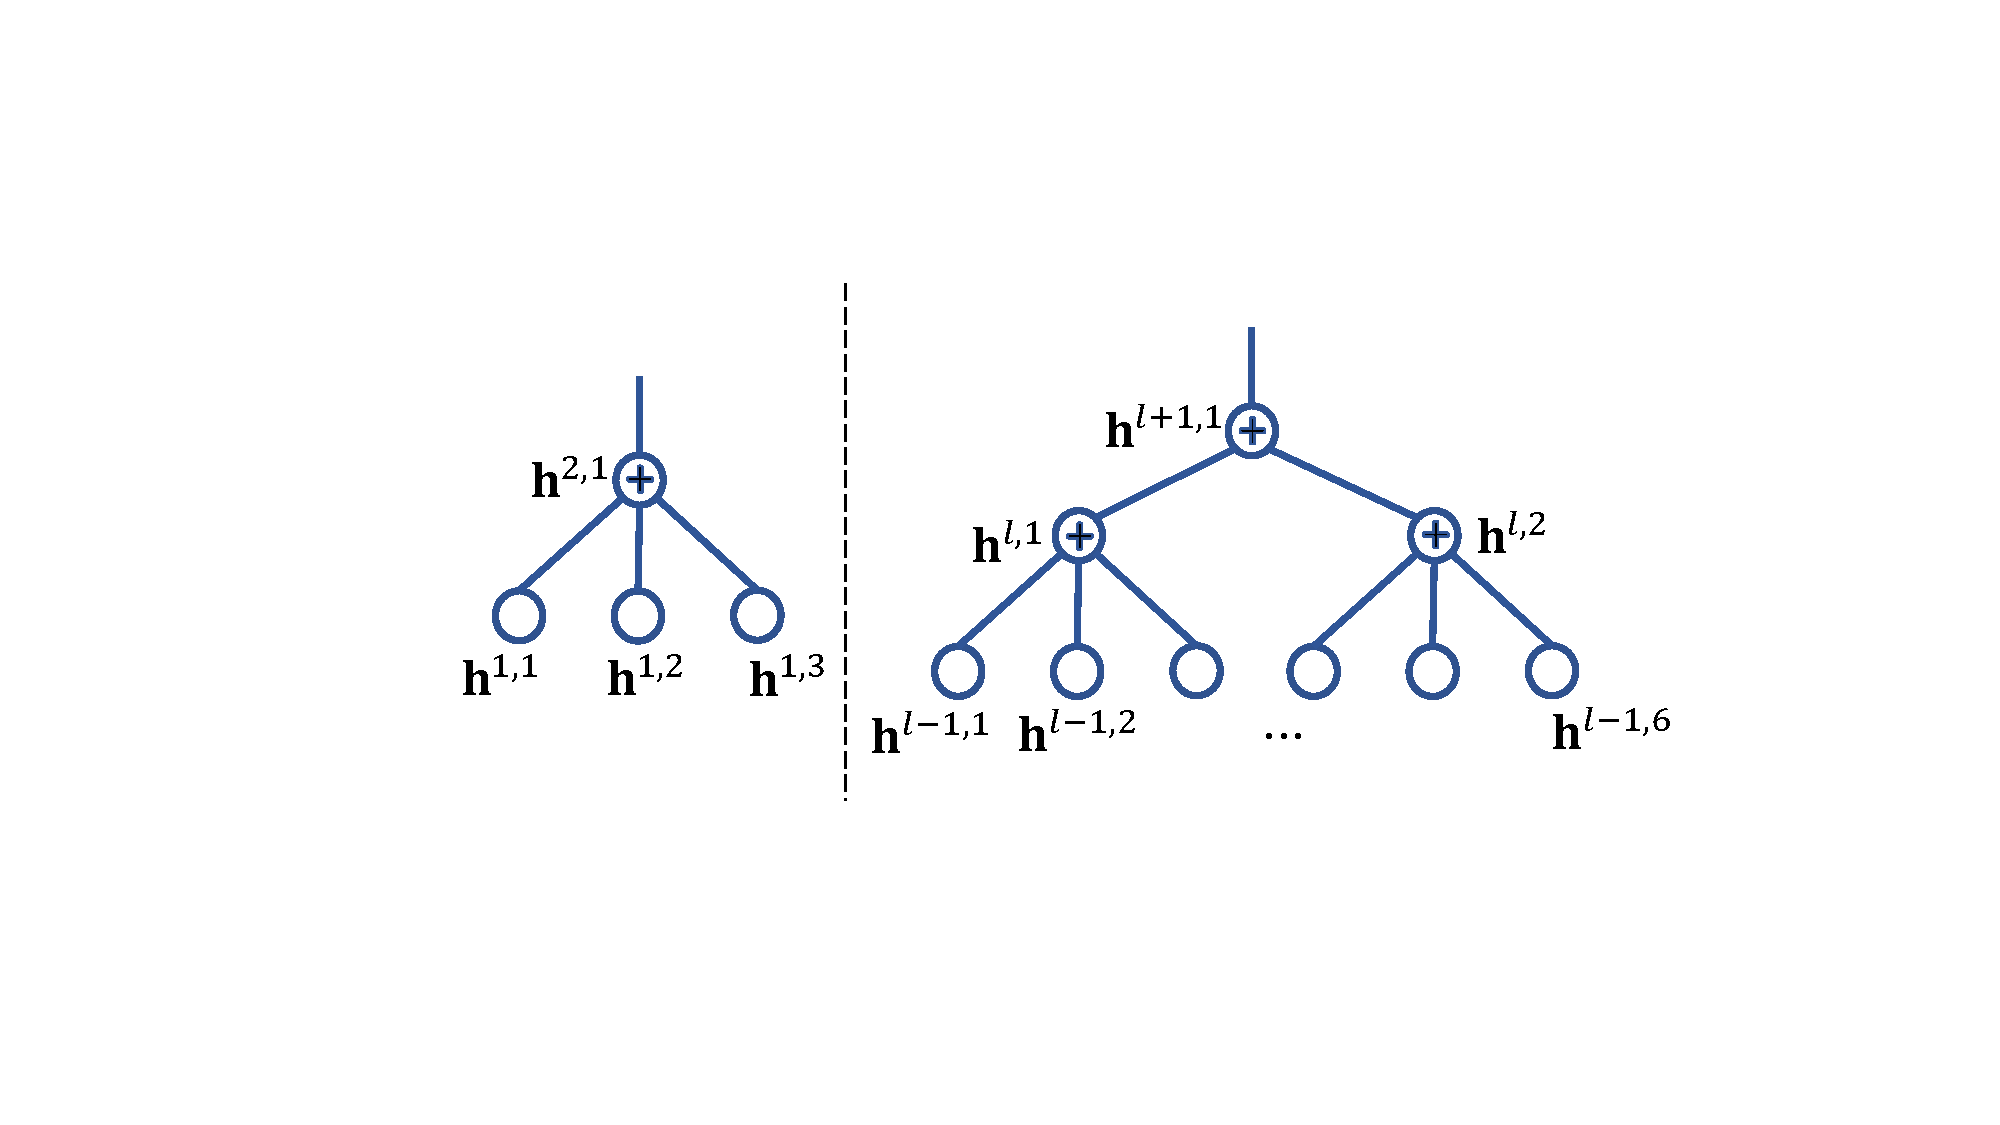
\includegraphics[width=1.0\linewidth]{fig/node.pdf}
\end{center}
\vspace{-0.2in}
\caption{ {\small (Left) The structure of one node. Node $\mathbf{h}^{2, 1}$ connects with its children with invertible functions. The messages from its children are aggregated at $\mathbf{h}^{2,1}$. (Right) An illustration of the latent structure from layer $l-1$ to $l+1$.  
$\mathbf{h}^{l, i}$ means the $i$th latent variable  in layer $l$.}}
\label{fig:node_tree}
\vspace{-0.15in}
\end{wrapfigure}
As shown in Figure~\ref{fig:node_tree}-(Left), a node in a flow-graph can have multiple children and multiple parents.
Each node has the forward messages from the input data samples and the backward messages from the root.  
If all the nodes only have one parent, then the structure becomes a tree. 
If there several nodes have multiple parents, the graph will be a DAG. 
It is easy to extend the computation of the ELBO~(\ref{eq:elbo_tree}) to DAGs with topology ordering of the nodes and thus the layer number. 
The ELBO for a DAG structure reads:
\begin{align}  \notag
 \log p(\mathbf{x}) \geqslant \mathcal{L}(\mathbf{x}; \theta_{\mathbf{f}}) 
= &  \sum_{i \in \mathcal{V}  \setminus  \mathcal{R}_{ \mathcal{G} }  }  \mathbb{E}_{q(\mathbf{h}^{pa(i)}|\mathbf{h}^{ch(pa(i))})} \bigg[ \log p( \mathbf{h}^{(i)}|  \widehat{\mathbf{h}}^{pa(i)})   \bigg]\\
 & +  \sum_{i \in \mathcal{V}  \setminus  \mathcal{R}_{ \mathcal{G} }  } \textbf{\text{H}}(\mathbf{h}^{(i)} | \mathbf{h}^{ch(i)} )   -    \sum_{i \in  \mathcal{R}_{ \mathcal{G} }  }  \textbf{\text{KL}}\big(q(\mathbf{h}^{(i)} | \mathbf{h}^{ch(i)} )   | p(\mathbf{h}^{(i)})  \big) . \label{eq:elbo_dag}
 \end{align}
Here $\mathcal{V}$ stands for the node set of DAG $\mathcal{G} = \{\mathcal{V}, \mathbf{f}\}$, and $\mathcal{R}_{ \mathcal{G}}$ is the set of root or source nodes. 
 
\begin{wrapfigure}[13]{r}{.25\textwidth}
\begin{center}
 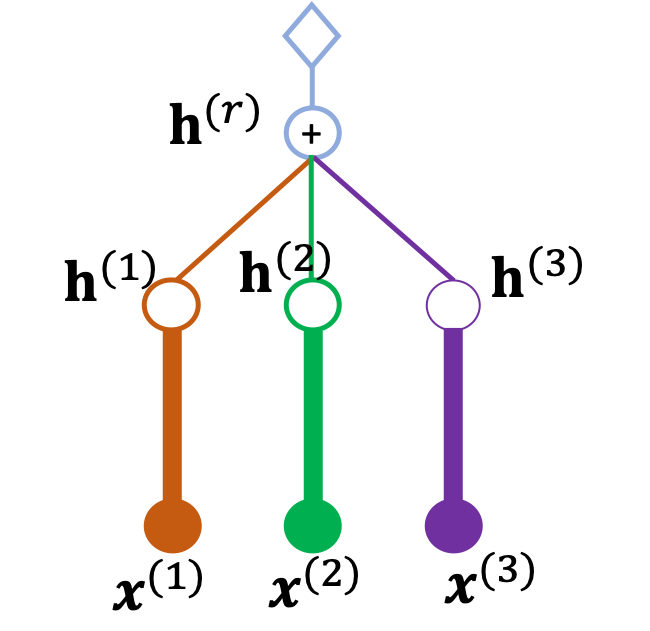
\includegraphics[width=1.0\linewidth]{fig/node_aggre_avg.png}
 %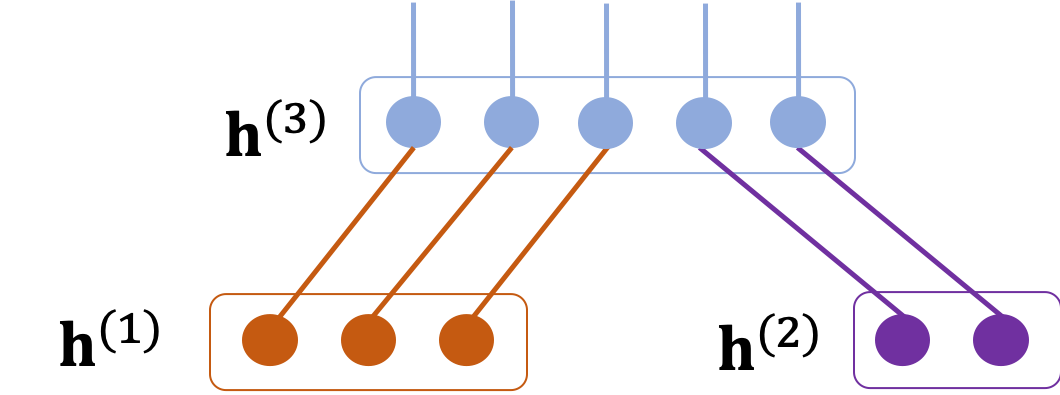
\includegraphics[width=0.43\linewidth]{fig/node_aggre_cat.png}
\end{center}
   \caption{Aggregation with average. $\mathbf{h}^{(r)}$ has three children, $\mathbf{h}^{(1)}$, $\mathbf{h}^{(2)}$, and $\mathbf{h}^{(3)}$.}
\label{fig:node_aggre}
\end{wrapfigure}

Assume there are $k$ leaf nodes on a tree or a DAG model, and they correspond to $k$ sections of the input sample $\mathbf{x} = [\mathbf{x}^{(1)}, ..., \mathbf{x}^{(k)}]$, then the hidden variables in both~(\ref{eq:elbo_tree}) and~(\ref{eq:elbo_dag}) are computed with forward and backward message passing. 
We provide more details about the nodes in next subsection.

\subsection{Node Aggregation}

In the sequel, we consider that all nodes latent variables, noted $\mathbf{h}^{l, i}$, for all $l [L]$ and $i \in \mathbb{N}$, admit Gaussian distributions as prior distribution.
There are two approaches to aggregate signals from different nodes:  \textsc{--} Average-based and \textsc{--} Concatenation-based  aggregation.
While concatenation-based aggregation is simple and straightforward, we rather focus on Average-based aggregation, cf. Figure~\ref{fig:node_aggre}, in this paper. 
We assume each entry of a hidden node follows a normal distribution, i.e., $\mathbf{h}_j^{(i)} \sim \mathcal{N}(\mu_j^{(i)}, \sigma^2)$ for node $i$'s $j$th entry. 
To avoid cumbersome notations, we  use the same standard deviation $\sigma$ across all nodes. 
Extending to different values for each node does not affect the rest of the paper.
Assume a model only has one average aggregation node as shown in Figure~\ref{fig:node_aggre}, then (\ref{eq:elbo_tree}) yields
\begin{align} \notag
\log p(\mathbf{x})  \geqslant \mathcal{L}(\mathbf{x}; \theta_{\mathbf{f}})
=&\mathbb{E}_{q(\mathbf{h}^1 | \mathbf{x})} \big[\log p(\mathbf{x}|\widehat{\mathbf{h}}^1)\big] + \mathbf{H}(\mathbf{h}^1 | \mathbf{x})  \\ \label{eq:average}
&+\mathbb{E}_{q(\mathbf{h}^2 | \mathbf{h}^1)} \big[\log p(\mathbf{h}^1|\widehat{\mathbf{h}}^2)\big] - \textbf{\text{KL}}\big(q(\mathbf{h}^2 | \mathbf{h}^1) | p(\mathbf{h}^2)\big).
\end{align} 
There are two aggregation rules for node $i$: (a) the parent value is the mean of its children, i.e., $\mathbf{h}^{(i)} = \frac{1}{|ch(i)|} \sum_{j \in ch(i)} \mathbf{h}^{(j)}$; (b) the  children have the same reconstruction value with its parent, i.e., $\widehat{\mathbf{h}}^{(j)} = \widehat{\mathbf{h}}^{(i)}, \forall j \in ch(i)$. 
% Here we give an example with a model that has only  one aggregation node.  
Consider a single aggregation node model.
Let $\mathbf{h}^{(r)}$ be the root, and it has $k$ children, $\mathbf{h}^{(t)}, t = 1,...,k$. 
With $\mathbf{f}_t$ as the flow function connecting $\mathbf{h}^{(t)}$ and $\mathbf{x}^{(t)}$, according to the aggregation rules we represent, in Figure~\ref{fig:node_aggre} with $k=3$, the following identities:
$$ \mathbf{h}^{(t)} = \mathbf{f}_t(\mathbf{x}^{(t)}),\quad \widehat{\mathbf{h}}^{(r)} = \mathbf{h}^{(r)} = \frac{1}{k}\sum_{t=1}^k \mathbf{h}^{(t)}, \quad \textrm{and} \quad  \widehat{\mathbf{h}}^{(t)}= \widehat{\mathbf{h}}^{(r)}, \ t = 1,...,k \, .$$
% Given a sample $\mathbf{x}$ and since $\widehat{\mathbf{h}}^{2}= \widehat{\mathbf{h}}^{(r)}$ and $\widehat{\mathbf{h}}^{(t)}= \widehat{\mathbf{h}}^{(r)} $, the reconstruction terms in (\ref{eq:average}) are~computed~with
Given a sample $\mathbf{x}$, the reconstruction terms in (\ref{eq:average}) are~computed~with
% \begin{align}\label{eq:yllk}
\begin{align}\notag
\log p(\mathbf{x}|\widehat{\mathbf{h}}^1) + \log p(\mathbf{h}^1|\widehat{\mathbf{h}}^2) =-\sum_{t=1}^k\bigg\{ \underbrace{\frac{1}{2\sigma^2_{\mathbf{x}}}\big|\big| \mathbf{x}^{(t)} - \mathbf{f}_t^{-1}(\widehat{\mathbf{h}}^{(r)})\big|\big|^2 }_{\textrm{By} \  \widehat{\mathbf{x}}^{(t)}=\mathbf{f}_t^{-1}(\widehat{\mathbf{h}}^{(t)})=\mathbf{f}_t^{-1}(\widehat{\mathbf{h}}^{(r)})} +  \underbrace{\frac{1}{2\sigma^2}\big|\big|  \mathbf{f}_t(\mathbf{x}^{(t)}) - \widehat{\mathbf{h}}^{(r)}\big|\big|^2}_{\textrm{By} \  \widehat{\mathbf{h}}^{2}= \widehat{\mathbf{h}}^{(r)}, \  \mathbf{h}^{(t)} = \mathbf{f}_t(\mathbf{x}^{(t)})} \bigg\} +C
\end{align} 

% \begin{align}\notag
% &\log p(\mathbf{x}|\widehat{\mathbf{h}}^1) + \log p(\mathbf{h}^1|\widehat{\mathbf{h}}^2)
% =-\sum_{t=1}^k\bigg\{ \underbrace{\frac{1}{2\sigma^2_{\mathbf{x}}}\big|\big| \mathbf{x}^{(t)} - \mathbf{f}_t^{-1}(\widehat{\mathbf{h}}^{(t)})\big|\big|^2}_{\textrm{By} \  \widehat{\mathbf{x}}^{(t)}=\mathbf{f}_t^{-1}(\widehat{\mathbf{h}}^{(t)})} +  \underbrace{\frac{1}{2\sigma^2}\big|\big| \mathbf{h}^{(t)} -\widehat{\mathbf{h}}^{(r)} \big|\big|^2}_{\textrm{By} \  \widehat{\mathbf{h}}^{2}= \widehat{\mathbf{h}}^{(r)}} \bigg\} +C \\
% &\hspace{1.3in}-\sum_{t=1}^k\bigg\{ \underbrace{\frac{1}{2\sigma^2_{\mathbf{x}}}\big|\big| \mathbf{x}^{(t)} - \mathbf{f}_t^{-1}(\widehat{\mathbf{h}}^{(r)})\big|\big|^2 }_{\textrm{By} \  \widehat{\mathbf{h}}^{(t)}= \widehat{\mathbf{h}}^{(r)} } +  \frac{1}{2\sigma^2}\big|\big|  \mathbf{f}_t(\mathbf{x}^{(t)}) - \widehat{\mathbf{h}}^{(r)}\big|\big|^2 \bigg\} +C \label{eq:yllk} .
% \end{align} 
Here $C=-dk\ln(2\pi)-\frac{dk}{2}\ln(\sigma_{\mathbf{x}}^2)-\frac{dk}{2}\ln(\sigma^2)$. We use constant values for both  $\sigma^2_{\mathbf{x}}$ and $\sigma^2$, hence the value of $C$ is constant as well. We use the latent variables from a batch of training samples to approximate the entry \textbf{H} and \textbf{KL} terms in~(\ref{eq:average}). We can see that maximizing the ELBO will force the average aggregation node to satisfy aggregation rule (b). We take the parent and children involved an aggregation operation as one node in the graphical figures, e.g., Figure~\ref{fig:node_tree}. 


\subsection{Inference on Sub-graphs }



\begin{wrapfigure}[12]{r}{.6\textwidth}
\vspace{-0.7in}
\begin{center}
 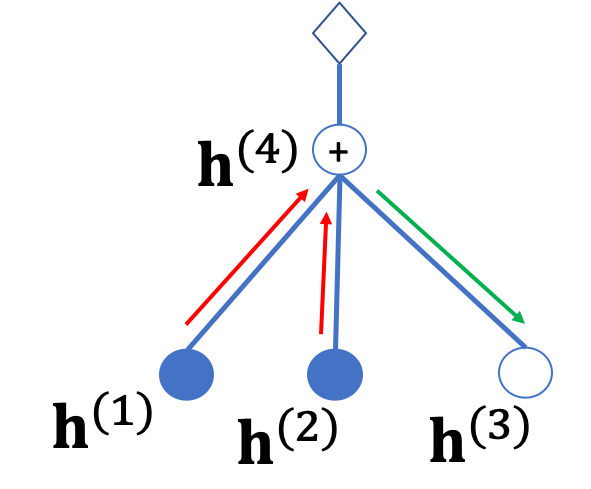
\includegraphics[width=0.4\linewidth]{fig/two_layer_infer.png}
 \hspace{0.15in}
 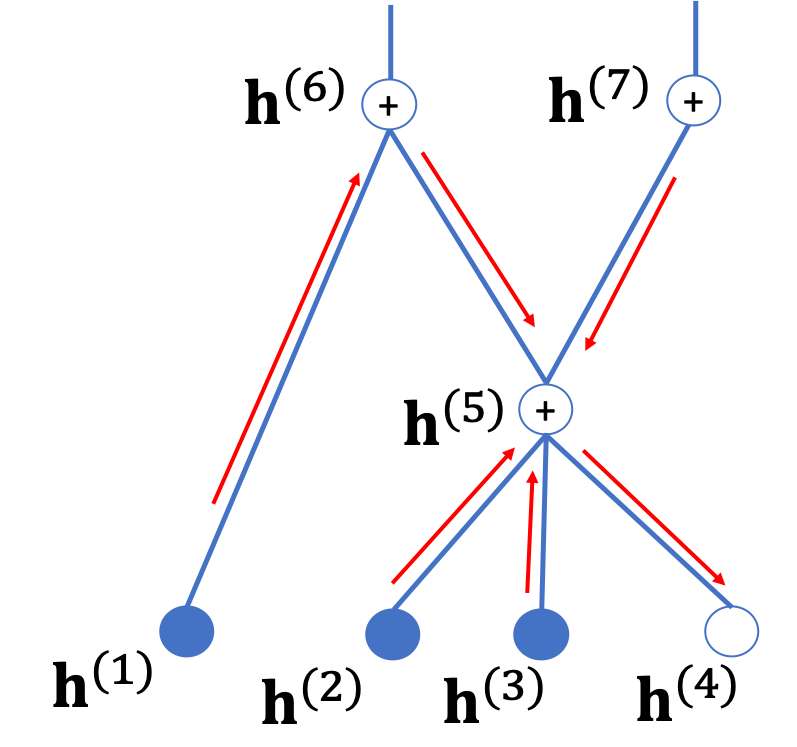
\includegraphics[width=0.5\linewidth]{fig/dag_infer.png}
\end{center}
\vspace{-0.1in}
 \caption{{\small (Left) Inference of single aggregation node model. Node 4 aggregates from node 1 and 2, and  pass the updated state to node 3 for prediction. (Right) Inference on a tree model. Observed node states are gathered in node 5 to predict the state of node 4.}}
\label{fig:two_layer_infer}
\end{wrapfigure}
Given a trained VFG model, we can infer the state of a node given the observed nodes. 
Relations between variables at different nodes can also be inferred via our flow-based graphical model. 
The hidden state of the parent node $j$ in a single aggregation model can be approximated by the observed children,
$\mathbf{h}^{(j)}  = \frac{1}{|ch(j)|}\sum_{i \in ch(j) \cap O} \mathbf{h}^{(i)}$ where $O$ is the set of observed leaf nodes, see Figure~\ref{fig:two_layer_infer}-left for an illustration. 
Observe that for either a tree or a DAG, the state of any given node is updated via messages received from its children. 
The message passing firstly occurs from the children to the parent with updating and then pass it back to the children without updating. 
Figure~\ref{fig:two_layer_infer} illustrates this inference mechanism for trees which structure enables to perform message passing among the nodes.  
We establish the following Lemma establishing the relation between two leaf nodes:
\begin{lemma}\label{lm:apprx}
Let $\mathcal{G}$ be a trained tree structured variational flow graphical model with $L$ layers, and $i$ and $j$ are two leaf nodes with $a$ as the closest common ancestor. Given observed value at node $i$, the value of node $j$ can be approximated by   $\widehat{\mathbf{x}}^{j} \approx  \mathbf{f}_{(a,j)}(\mathbf{f}_{(i, a)}(\mathbf{x}^{(i)}))$. Here $\mathbf{f}_{(i, a)}$ is the flow function path from node $i$ to node $a$. The conditional density of $\mathbf{x}^{(j)}$ given $\mathbf{x}^{(i)}$ can be approximated by: 
\begin{align} \label{eq:cond_llk}
\log p(\mathbf{x}^{(j)} | \mathbf{x}^{(i)}) &\approx  \log p(\widehat{\mathbf{h}}^L) -  \frac{1}{2} \log \big(\det \big(\mathbf{J}_{\widehat{\mathbf{x}}^{(j)}}(\widehat{\mathbf{h}}^L)^\top\mathbf{J}_{\widehat{\mathbf{x}}^{(j)}}(\widehat{\mathbf{h}}^L)\big) \big).
\end{align}
\end{lemma}
Rsing the normalizing flow~(\ref{eq:flow}), we have the following identity for each node of the graph structure:
\begin{align*}
p(\mathbf{h}^{(i)} | \mathbf{h}^{pa(i)}) & = p(\mathbf{h}^{pa(i)}) \big|\det(\frac{\partial \mathbf{h}^{pa(i)} }{\partial \mathbf{h}^{(i)}})\big| =
p(\mathbf{h}^{pa(i)}) \big|\det(\mathbf{J}_{\mathbf{h}^{pa(i)}}(\mathbf{h}^{(i)}))\big| .
\end{align*} 
% The proof of Lemma~\ref{lm:apprx} can be found in the appendix. 

\begin{remark}\label{rmk:apprx_mul}
Let $O$ be the set of observed leaf nodes, $j$ be an unobserved node, and $a$ the closest ancestor of $O \cup \{a\}$. Then the state of $j$ can be imputed with $\widehat{\mathbf{x}}^{j} \approx  \mathbf{f}_{(a,j)}(\mathbf{f}_{(O, a)}(\mathbf{x}^{(i)}))$, where $\mathbf{f}_{(O, a)}$ is the flow function path from all nodes in $O$ to $a$, and approximation~(\ref{eq:cond_llk}) still holds for $p(\mathbf{x}^{(j)} | \mathbf{x}^{O})$.
\end{remark}
We note that these results can be easily extended to DAG models.


\subsection{Algorithm and Implementation}


In this section, we develop the training algorithm, see Algorithm~\ref{alg:main}, that outputs the fitted vector of parameters resulting from the maximization of the ELBO objective function~(\eqref{eq:elbo_tree}) or~(\eqref{eq:elbo_dag}) depending on what graph structure is used.
In Algorithm~\ref{alg:main}, the inference of the latent variables is performed via forward message passing, cf. Line~\ref{line:forward}, and their reconstructions are computed in backward message passing, cf. Line~\ref{line:backward}.

Different from VAE,  the variance of latent variables in a VFG are set with a fixed value rather than parameterized with neural networks. A VFG is a deterministic network passing latent variable values between nodes. The reconstruction~(likelihood) terms in each layer are computed with forward and backward node states. We use the empirical variance in a batch of training samples to approximate the entropy and \textbf{KL} terms. Ignoring  explicit neural network parameterized variances  for all latent nodes enable us to use flow-based models as the encoders as well as the decoders. It also helps the model to get rid of sampling steps and to obtain a deterministic ELBO objective~\eqref{eq:elbo_tree} and~\eqref{eq:elbo_dag} that can be efficiently optimized with standard stochastic solvers. 


\begin{algorithm}[H]
\algsetup{indent=0.25em}
   \caption{Inference model parameters with  forward and backward message propagation}
   \label{alg:main}
\begin{algorithmic}[1]
   \STATE {\bfseries Input:} Data distribution $\mathcal{D}$,  $\mathcal{G} = \{\mathcal{V}, \mathbf{f}\}$
   \FOR {$s=0,1,...$}
   \STATE  Sample minibatch $b$ samples $\{\mathbf{x}_1, ..., \mathbf{x}_b \}$ from $\mathcal{D}$;
   \FOR{$i \in \mathcal{V}$}
   \STATE $\mathbf{h}^{(i)} = \frac{1}{|ch(i)|} \sum_{j \in ch(i) } \mathbf{f}_{(j,i)}(\mathbf{h}^{(j)})$; \label{line:forward} \textcolor{blue}{// forward message passing}
    \ENDFOR
    \STATE $\widehat{\mathbf{h}}^{(i)} = \mathbf{h}^{(i)} \ \  \text{if} \ i \in \mathcal{R}_{\mathcal{G}} $ or $i \in$ layer L;
   \FOR{$i \in \mathcal{V}$}
   \STATE $\widehat{\mathbf{h}}^{(i)} = \frac{1}{|pa(i)|} \sum_{j \in pa(i) } \mathbf{f}^{-1}_{ (i,j)}(\widehat{\mathbf{h}}^{(j)}) $;\label{line:backward}  \textcolor{blue}{// backward message passing}
   \ENDFOR
    \STATE  $\mathbf{h} =  \{\mathbf{h}^{(1)}, ...,  \mathbf{h}^{(|\mathcal{V}|)}  \}$ and $ \widehat{\mathbf{h}} =  \{\widehat{\mathbf{h}}^{(1)}, ...,  \widehat{\mathbf{h}}^{(|\mathcal{V}|)}  \}$;
    \STATE Approximate the entropy $\mathbf{H}$ and $\mathbf{KL}$ terms in ELBO for each layer with b samples;
    \STATE Updating VFG model $\mathcal{G}$ with gradient ascending: $\theta^{(s+1)}_{\mathbf{f}} = \theta^{(s)}_{\mathbf{f}} + \nabla_{\theta_{\mathbf{f}}}\frac{1}{b} \sum_{i=1}^b  \mathcal{L}(\mathbf{x}_b; \theta^{(s)}_{\mathbf{f}})   \, .$
   %\ENDFOR 
   \ENDFOR
\end{algorithmic}
\end{algorithm}

% \begin{algorithm}[H]
% \algsetup{indent=0.25em}
%   \caption{Inference model parameters with  forward and backward message propagation}
%   \label{alg:main}
% \begin{algorithmic}[1]
%   \STATE {\bfseries Input:} Data distribution $\mathcal{D}$,  $\mathcal{G} = \{\mathcal{V}, \mathbf{f}\}$
%   \FOR {$s=0,1,...$}
%   \STATE  Sample minibatch $b$ samples $\{\mathbf{x}_1, ..., \mathbf{x}_b \}$ from $\mathcal{D}$;
%   \FOR{$i \in \mathcal{V}$}
%   \STATE $\mathbf{h}^{(i)} = \frac{1}{|ch(i)|} \sum_{j \in ch(i) } \mathbf{f}_{(j,i)}(\mathbf{h}^{(j)})$; \label{line:forward} \textcolor{blue}{// forward message passing}
%   \ENDFOR
%     \STATE  $\mathbf{h} =  \{\mathbf{h}^{(1)}, ...,  \mathbf{h}^{(|\mathcal{V}|)}  \}$;
%     \FOR{$i \in \mathcal{V}$}
%   \STATE $\widehat{\mathbf{h}}^{(i)} = \frac{1}{|pa(i)|} \sum_{j \in pa(i) } \mathbf{f}^{-1}_{ (i,j)}(\widehat{\mathbf{h}}^{(j)}) $;\label{line:backward}  \textcolor{blue}{// backward message passing}
%   \ENDFOR
%     \STATE  $ \widehat{\mathbf{h}} =  \{\widehat{\mathbf{h}}^{(1)}, ...,  \widehat{\mathbf{h}}^{(|\mathcal{V}|)}  \}$;
    
%     \STATE Approximate the entry $\mathbf{H}$ and $\mathbf{KL}$ terms in ELBO for each layer with b samples;
%     \STATE Updating flow-graph $\mathcal{G}$ using SGD: $\theta^{(k+1)} = \theta^{(k)} -  \nabla_{\theta}\frac{1}{b} \sum_{i=1}^b  \mathcal{L}(\mathbf{x}_b; \theta^{(k)})   \, .$
%   %\ENDFOR 
%   \ENDFOR
% \end{algorithmic}
% \end{algorithm}


% Let's focus on a model that has only one aggregation node as shown in Figure~\ref{fig:node_aggre}-left.

\section{Theory}\label{sec:theory}


The proposed VFG models provide approaches to integrate multi-modal data or data sets from different sources. With  invertible flow functions, we try to analyse the identifiability~\citep{Khemakhem20a,Sorrenson2020} of the VFG in this subsection.  We assume each data sample has $k$ sections, and $\mathbf{h}^{(t)}$ is the latent variable for section $t$, $\mathbf{x}^{(t)}$. Suppose the distribution regarding latent variable $\mathbf{h}^{(t)}$ is a factorial member of the exponential family with $m$ sufficient statistics, conditioned on $\mathbf{u}$. Here $\mathbf{u}$ is additional observed variable. The general form of the distribution can be written as 
\begin{equation}\label{eq:exp_h}
p_{\mathbf{h}^{(t)}}(\mathbf{h}^{(t)} | \mathbf{u}) = \Pi_{i=1}^d \frac{Q_i(h^{(t,i)})}{Z_i(\mathbf{u})} \text{exp}\bigg[ \sum_{j=1}^m T_{i,j}(h^{(t,i)}) \lambda_{i,j}(\mathbf{u}) \bigg].
\end{equation} 
Here $Q_i$ is the base measure, $Z_i(\mathbf{u})$ is the normalizing constant, $T_{i,j}$ are the component of the sufficient statistic and $\lambda_{i,j}$ the corresponding parameters,  depending on $\mathbf{u}$. Variable $\mathbf{x}^{(t)}$ is generated with some complex, invertible, and deterministic  function from the latent space: $\mathbf{x}^{(t)} = \mathbf{f}^{-1}_t(\mathbf{h}^{(t)}, \epsilon)$. Let $\mathbf{T} =[\mathbf{T}_1, ..., \mathbf{T}_l] $, and $\mathbf{\lambda} =[\mathbf{\lambda}_1, ..., \mathbf{\lambda}_l]$.  We define the domain of $\mathbf{f}_t^{-1}$ as $\mathcal{H}=\mathcal{H}_1 \times ... \times \mathcal{H}_l$.
Here $Q_i$ is the base measure, $Z_i(\mathbf{u})$ is the normalizing constant, $T_{i,j}$ are the component of the sufficient statistic and $\lambda_{i,j}$ the corresponding parameters,  depending on $\mathbf{u}$. Variable $\mathbf{x}^{(t)}$ is generated with some complex, invertible, and deterministic  function from the latent space: $\mathbf{x}^{(t)} = \mathbf{f}^{-1}_t(\mathbf{h}^{(t)}, \epsilon)$. Let $\mathbf{T} =[\mathbf{T}_1, ..., \mathbf{T}_l] $,  $\mathbf{\lambda} =[\mathbf{\lambda}_1, ..., \mathbf{\lambda}_l]$, and $\Theta = \{\mathbf{\theta} := (\mathbf{T}, \mathbf{\lambda}, \mathbf{f}^{-1}_k)\}$.  We define the domain of $\mathbf{f}_t^{-1}$ as $\mathcal{H}=\mathcal{H}_1 \times ... \times \mathcal{H}_l$. We use $\widehat{\Theta} = \{\widehat{\mathbf{\theta}} := (\widehat{\mathbf{T}}, \widehat{\mathbf{\lambda}}, \mathbf{g}\}$ to represent the model learned by a piratical algorithm.
In the limit of infinite data and perfect convergence, we have the following theorem regarding the identifiability of $\mathbf{T}$. 

\begin{theorem}\label{thm:identif}
Assume we observe data distributed according to the generative model given by~\eqref{eq:exp_h} and $\mathbf{x}^{(t)} = \mathbf{f}^{-1}_t(\mathbf{h}^{(t)}, \epsilon)$, we further have the following assumptions,

\vspace{0.05in}

(a) The sufficient statistics $T_{ij}(h)$ are differentiable almost everywhere and their derivatives $\frac{d T_{i,j}}{d h}$ are nonzero almost surely for all $h\in \mathcal{H}_i$ and all $1\leq i \leq d$ and $1 \leq j  \leq m$.

\vspace{0.05in}


(b) There exist $dm+1$ distinct conditions $\mathbf{u}^{(0)}$, ..., $\mathbf{u}^{(dm)}$  such that the matrix 
\begin{equation*} 
\mathbf{L} = [\mathbf{\lambda}(\mathbf{u}^{(1)}) - \mathbf{\lambda}(\mathbf{u}^{(0)}), ..., \mathbf{\lambda}(\mathbf{u}^{(dm)}) - \mathbf{\lambda}(\mathbf{u}^{(0)}) ]
\end{equation*} 
of size $dm \times dm$ is invertible.
Then the model parameters 
$\mathbf{T}(\mathbf{h}_k) = \mathbf{A}\widehat{\mathbf{T}}(\mathbf{h}_k) + \mathbf{c}.$ Here $\mathbf{A}$ is an $dm \times dm$ invertible matrix and $\mathbf{c}$ is a vector of size $dm$.
\end{theorem}

% The proof of Theorem~\ref{thm:identif} and further analysis can be found in the appendix. 


\section{Numerical Experiments}\label{sec:numerical}


We present in this section several numerical experiments to highlight the benefits of our VFG model.
The first main application we present consists in missing values imputation. Several baseline models are compared with our newly introduced one on both synthetic and real datasets.
The second application we present is to learn the disentangled latent representations   that separate the explanatory factors of variations in the data, see~\citet{bengio2013representation}.
For that latter application, the model is trained and evaluated on the MNIST handwritten digits dataset.


\subsection{Missing entries imputation}

We now focus on the task of imputing missing entries in a graph structure.
For all the following experiments, the models are trained on the training set and are used to infer the missing entries of samples in the testing set.

\textbf{Baseline Methods:} We use the following baselines for data imputation:\vspace{-0.05in}
\begin{itemize}
\item \textit{Mean Value:} Using training set mean values to replace the missing entries in the testing set.   
\item \textit{Iterative Imputation:} A strategy for imputing missing values by modeling each feature with missing values as a function of other features in a Round-Robin fashion.   
% We choose the KNeighborRegressor as the specific function~\citep{scikit-learn}.

\item \textit{KNN:} To use K-Nearest Neighbor for data imputation,  we compare the non-missing entries of each sample to the training set and use the  average of top $k$ samples as imputation values   

\item \textit{Multivariate Imputation by Chained Equation (MICE):} This method impute the missing entries with multiple  rounds of inference. This method can handle different type of data.
\end{itemize}  

\textbf{Evaluation with Synthetic Data: }
In this set of experiments, we study the proposed model with synthetic datasets.
We generate a synthetic dataset of $1\,300$ data points, $1\,000$ for the training phase of the model, $300$ for imputation testing. Each data sample  has $8$ dimensions with $2$ latent variables. Let $z_1 \sim \mathcal{N}(0,1.0^2)$ and $z_2 \sim  \mathcal{N}(1.0,2.0^2)$ be the latent variables. For a sample $\mathbf{x}$, we have  $x_1=x_2 = z_1, x_3=x_4= 2.0\textrm{sin}(z_1), x_5=x_6 =z_2$, and $x_7= x_8 = z_2^2$.  In the testing dataset, $x_3$, $x_4$, $x_7$, and $x_8$ are missing. We use a VFG model with a single average aggregation node that has 4 children, and each child connects the parent with a flow function consists of 3 coupling layers\citep{Dinh2016DensityEU}. Each child takes 2 variables as input data section, and the latent dimension of the VFG is 2.  Table~\ref{tab:imp} presents the imputation MSE values through different methods.
Figure~\ref{fig:elbo} gives the ELBO values of the proposed method. 

 \begin{minipage}{\textwidth}
  \begin{minipage}[b]{0.49\textwidth}
    \centering
   \includegraphics[width=2.1in]{fig/sim_elbo.eps}
    \captionof{figure}{ELBO on the synthetic data}
    \label{fig:elbo}
  \end{minipage}
  \hfill
  \begin{minipage}[b]{0.49\textwidth}
    \centering
 \begin{tabular}{l | c  }\hline
Methods & Imputation MSE  \\
\hline
Mean Value &8.43 \\
\hline
MICE &8.24 \\
\hline
Iterative Imputation & 2.64 \\
\hline
KNN (k=3) &0.14 \\
\hline
KNN (k=5) &0.18 \\
\hline
Proposed &  1.45  \\  
\hline
\end{tabular}
\vspace{0.4in}
\captionof{table}{Imputation Results on Synthetic Data.} \label{tab:imp}
\end{minipage}
\end{minipage}  
  
%\begin{figure}[!htbp]
%    \centering
%    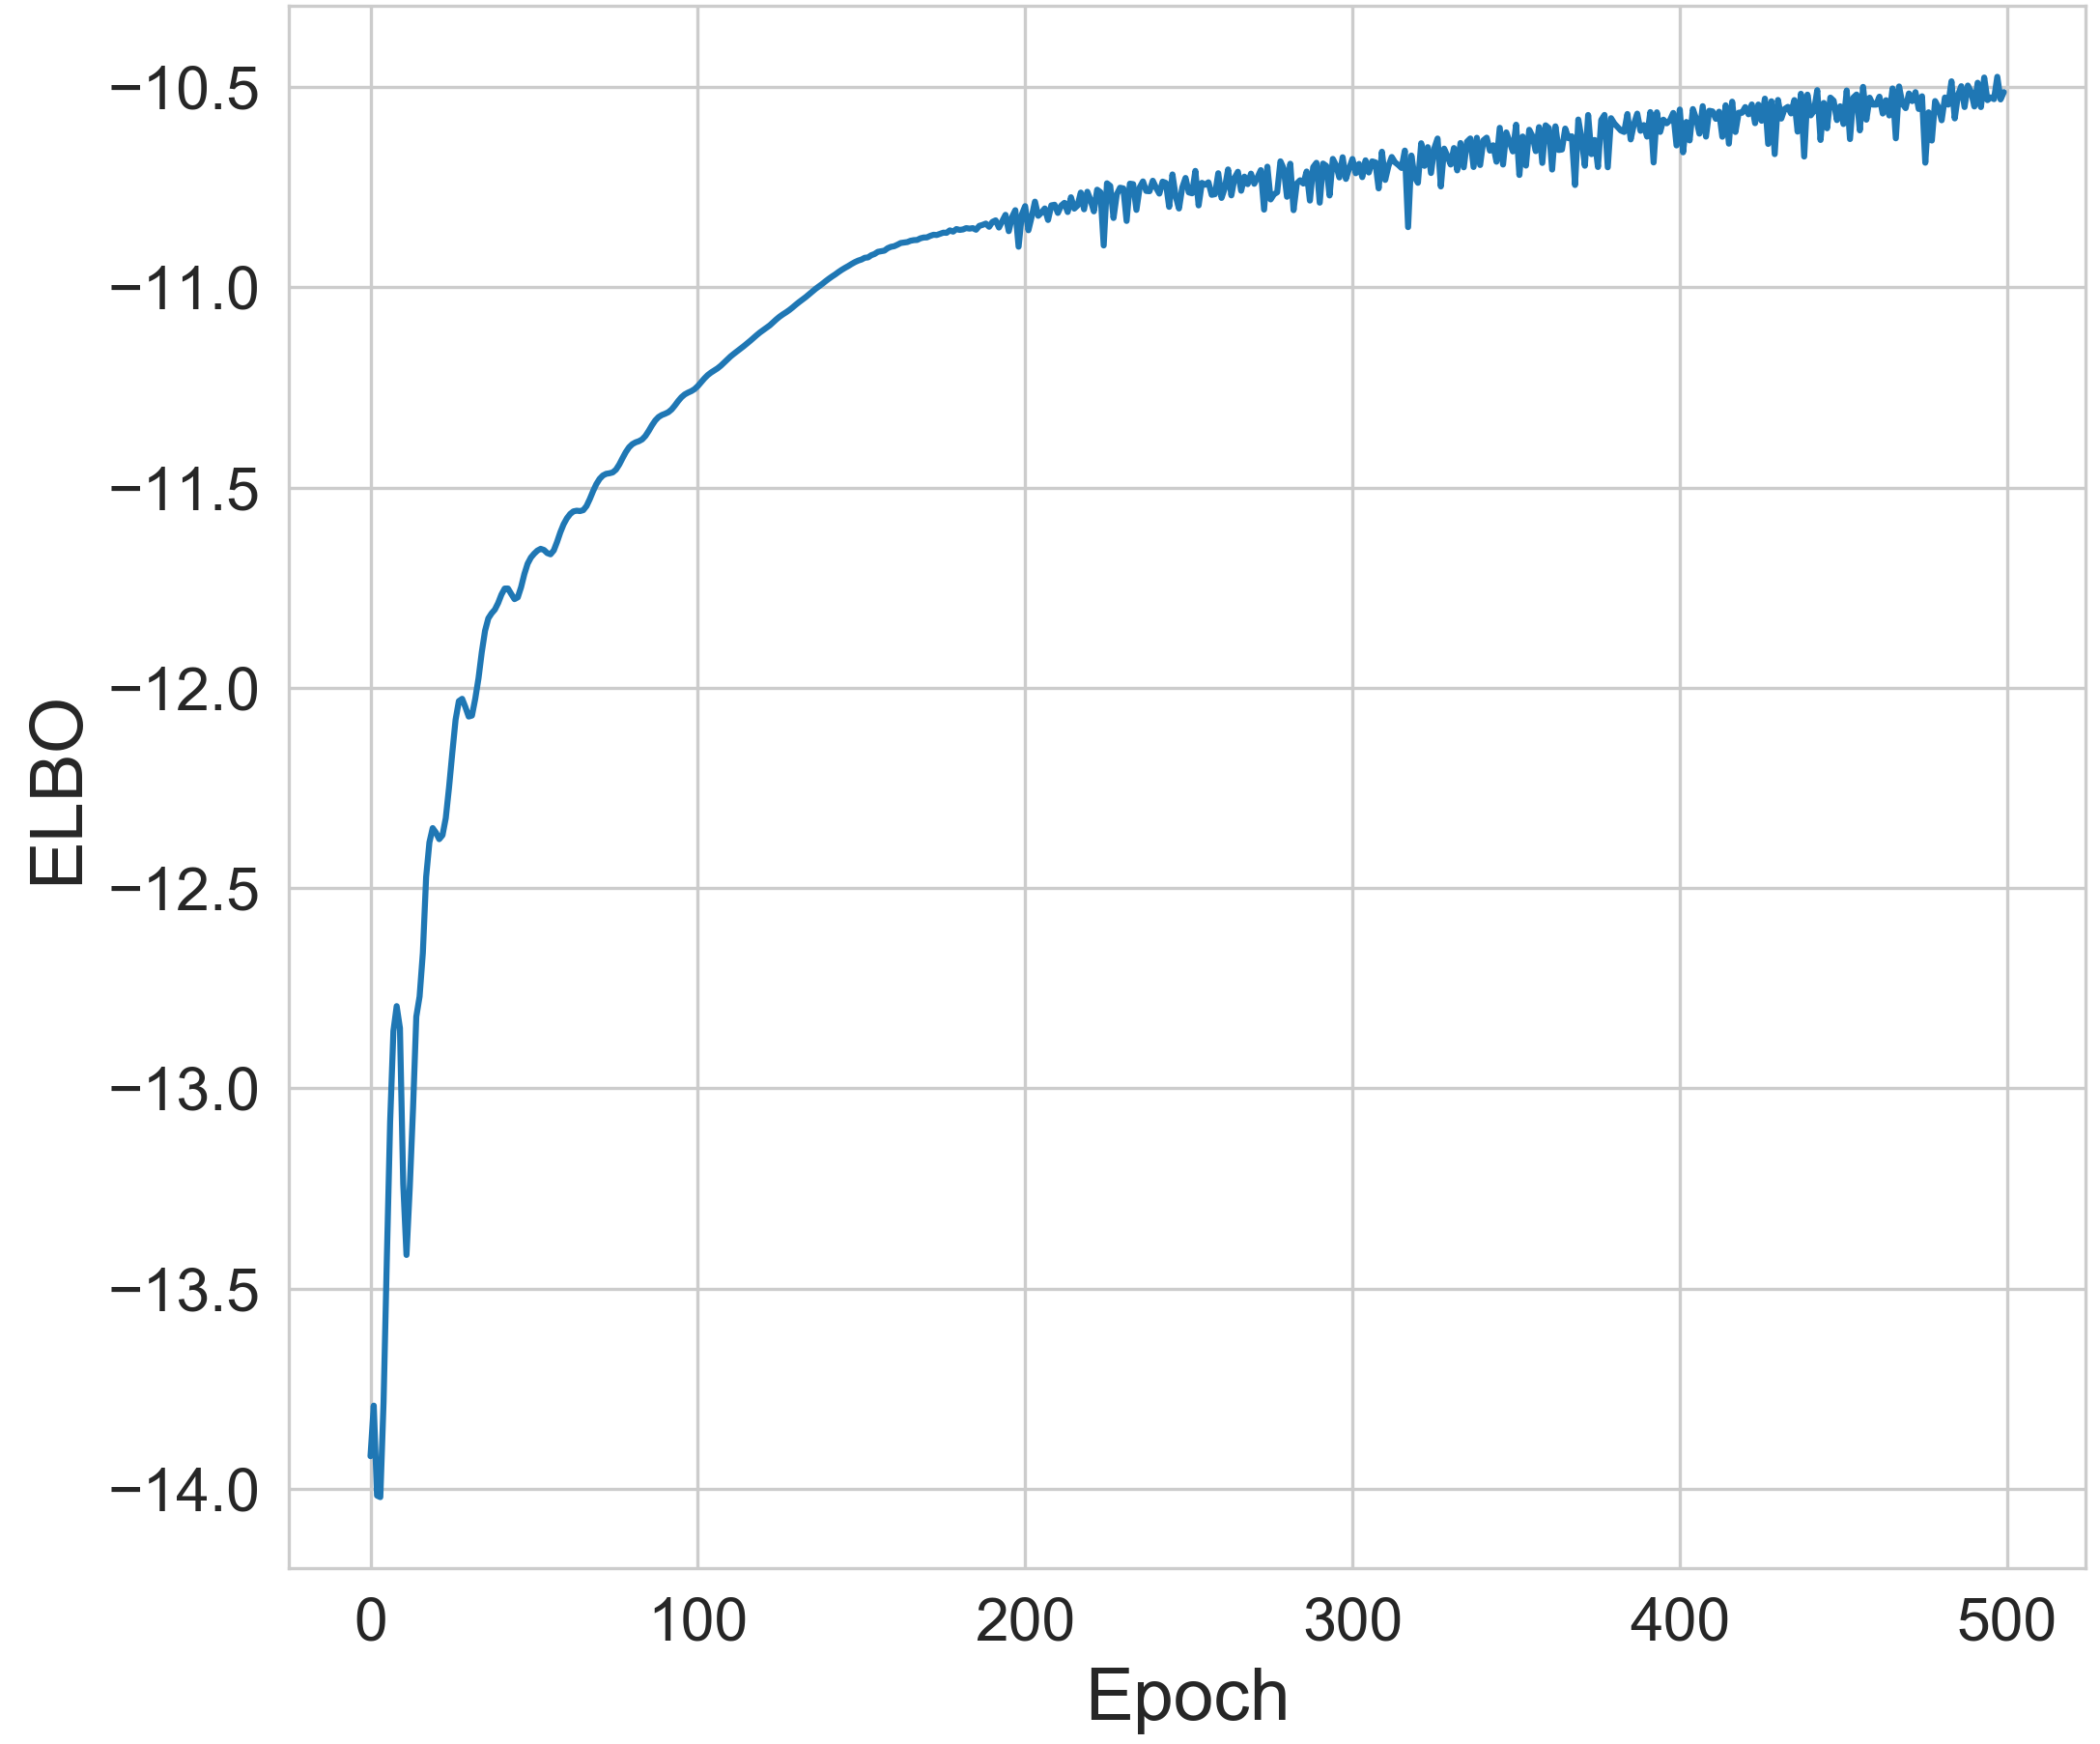
\includegraphics[width=2.3in]{fig/elbo.png}
%    \caption{ELBO on the synthetic data}
%    \label{fig:elbo}
%\end{figure}

% \begin{figure*}[!htbp]
%     \centering
%     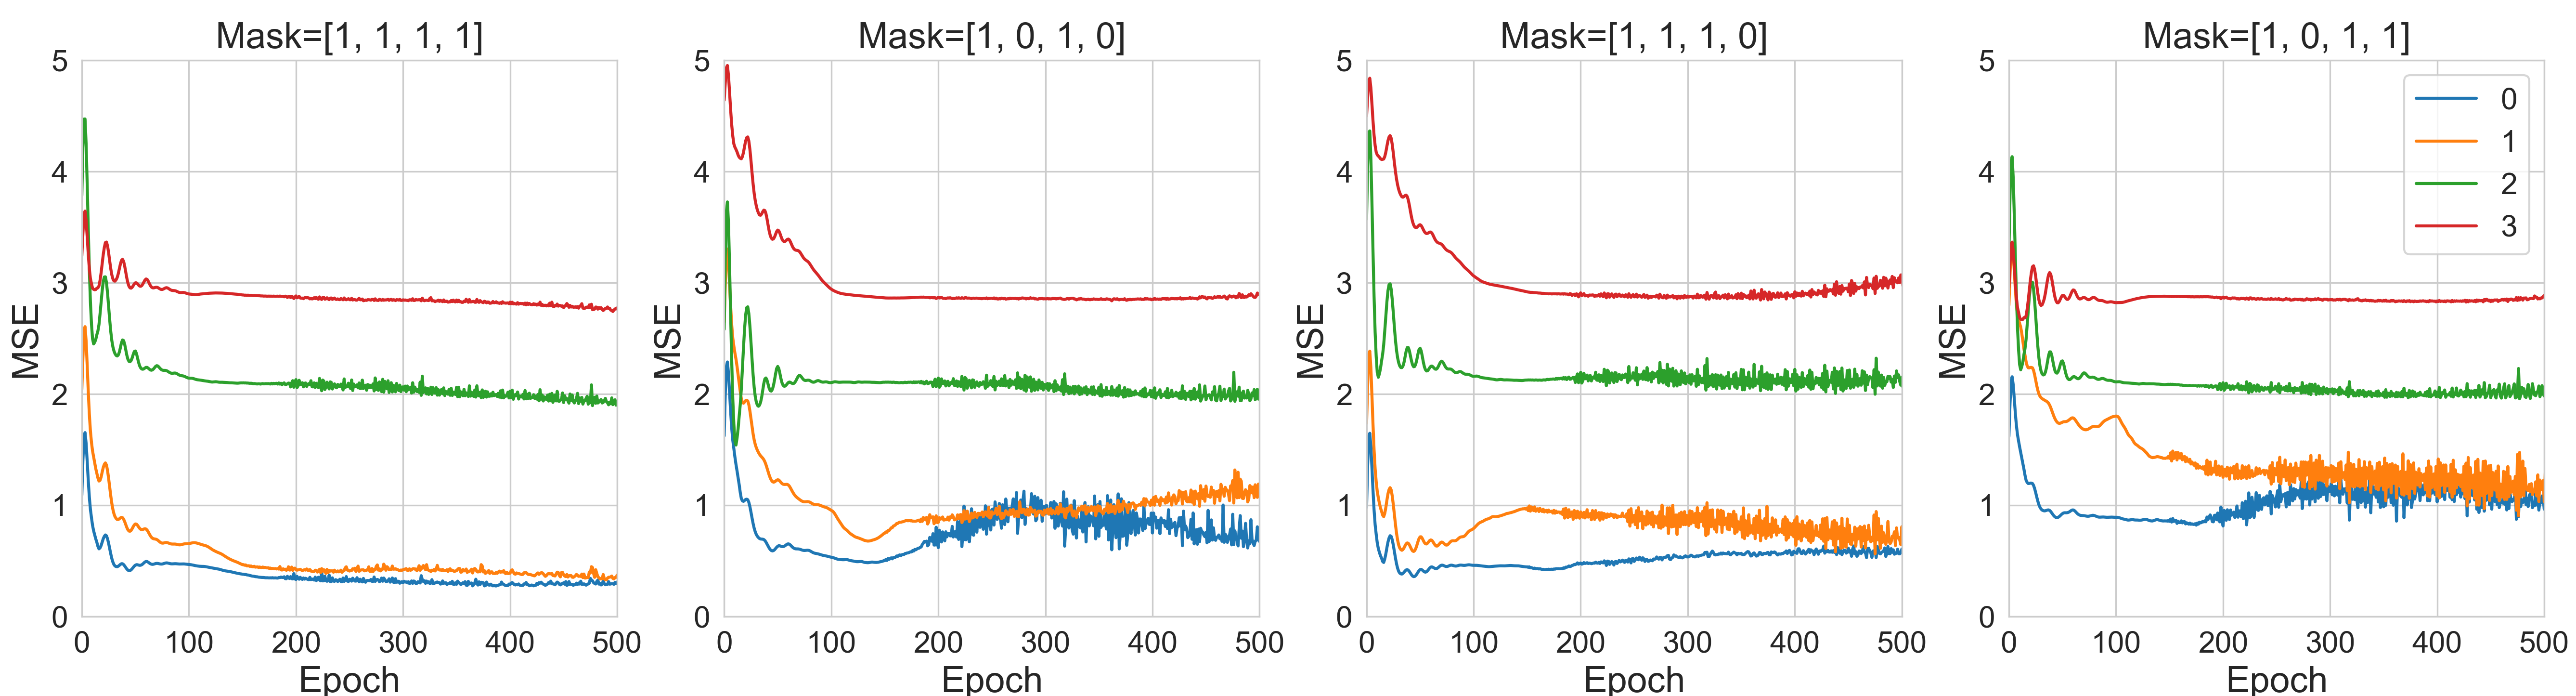
\includegraphics[width=0.95\textwidth]{fig/mse.png}
%     \caption{Imputation with $\mathsf{Mask}$ on the child nodes [0, 1, 2, 3] indicated by colored legends. }
%     \label{fig:mse}
% \end{figure*}

%\subsubsection{Data Imputation}

%\subsubsection{Graph Structure Recovery}


%
%
%    \begin{table}[t!]
%\begin{center}
%%\vspace{0.15in}
%\caption{Imputation Results on Synthetic Data.} \label{tab:causality2}
%\begin{tabular}{l | c  }\hline
%Methods & Imputation MSE  \\
%\hline
%Mean Value &8.43 \\
%\hline
%MICE &8.38 \\
%\hline
%Iterative Imputation & 2.64 \\
%\hline
%KNN (k=3) &0.14 \\
%\hline
%KNN (k=5) &0.18 \\
%\hline
%Proposed &  1.45  \\  
%\hline
%\end{tabular}
%\end{center}
%\end{table}


  
\textbf{Arrhythmia Dataset: }
We further investigate the method on a tabular dataset.  
The Arrhythmia~\citep{Dua:2019} dataset is  obtained from the ODDS repository. %The smallest classes, including 3, 4, 5, 7, 8, 9, 14, and 15, are combined to form the anomaly class, and the rest of the classes are combined to form the normal class. Table~\ref{tab:arrhythmiacausality2} shows the anomaly detection results with different methods. 


\subsection{Disentanglement on MNIST}

In this set of experiments, we evaluate disentanglement of VFGs on MNIST data. Disentanglement evaluation metrics have been proposed by~\cite{Karaletsos2015BayesianRL, Higgins17, Kim18, Eastwood18}.The authors of~\cite{Chen18} proposed to use the mutual information gap~(MIG) between latent variables and the ground truth factors to measure disentanglement.  In this paper, we resort to the approach proposed in~\citet{Eastwood18} for the following experiments. ~\cite{Eastwood18} studies a regression-based approach dividing the latent space data into training, evaluation, and testing. The disentanglement score is obtained based on the performance of the learned regression model. 


\section{Conclusion}\label{sec:conclusion}

In this paper, we propose VFG, a variational flow graphical model that integrates normalizing flows in the paradigm of graphical models.
Our VFG model learns the hierarchical latent structure of the input data through message passing between latent nodes. 
Experiments on missing data imputation and disentangled representation learning illustrate the effectiveness of the model. 
Future work includes applying our model to fine grained data relational structure learning and reasoning. 



% \section*{Acknowledgment}

% The preferred spelling of the word ``acknowledgment'' in America is without 
% an ``e'' after the ``g''. Avoid the stilted expression ``one of us (R. B. 
% G.) thanks $\ldots$''. Instead, try ``R. B. G. thanks$\ldots$''. Put sponsor 
% acknowledgments in the unnumbered footnote on the first page.

\clearpage
\bibliographystyle{iclr2021_conference}
\bibliography{references}

\clearpage
\section*{Appendix A.  ELBO of Tree Models}\label{appd:tree_elbo}

The hierarchy generative network as given in Figure~\ref{fig:tree-d}. For each pair of connected nodes, the edge is linked with an invertible function. We use $\theta$ to represent the parameters for all the edges.
The forward message passing starts from $\mathbf{x}$ and ends at $\mathbf{h}^L$, and backward message passing is in the reverse direction. 
 Then the
 likelihood for the data is given by
\begin{align*}
p(\mathbf{x}| \mathbf{\theta}) = \sum_{\mathbf{h}^1, ..., \mathbf{h}^L} p(\mathbf{h}^L | \theta)p(\mathbf{h}^{L-1} | \mathbf{h}^{L},\theta) \cdot \cdot  \cdot  p(\mathbf{x} | \mathbf{h}^{1}, \theta) .
\end{align*}

\begin{figure}[!htbp]
    \centering
    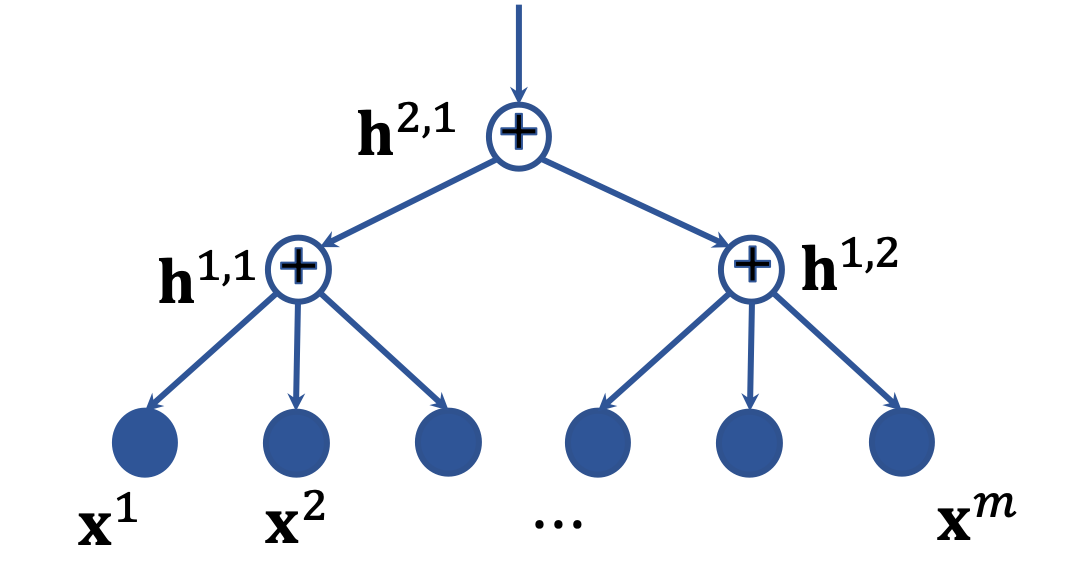
\includegraphics[width=2.3in]{fig/tree_direct.png}
    \caption{Tree structure.}
    \label{fig:tree-d}
\end{figure}

With the flow-based ensemble model, each edge is invertible.   The hierarchy of recognition network is the procedure from top to down of the structure as shown in Figure~\ref{fig:tree-d}.  Similarly, with the Markov property of the structure, the posterior density of the latent 
variables is given by
\begin{align*}
q(\mathbf{h}| \mathbf{x}, \theta ) = q(\mathbf{h}^1 | \mathbf{x}, \theta)  q(\mathbf{h}^2 | \mathbf{h}^1, \theta) \cdot \cdot  \cdot  q(\mathbf{h}^{L} | \mathbf{h}^{L-1}, \theta) \, ,
\end{align*}
which can be simplified as 
\begin{align*}
q(\mathbf{h}| \mathbf{x}) = q(\mathbf{h}^1 | \mathbf{x})  q(\mathbf{h}^2 | \mathbf{h}^1) \cdot \cdot  \cdot  q(\mathbf{h}^{L} | \mathbf{h}^{L-1}) \, .
\end{align*}
Note that we also have 
\begin{align} \label{eq:chain}
q(\mathbf{h}| \mathbf{x}) = q(\mathbf{h}^1 | \mathbf{x})  q(\mathbf{h}^{2:L} | \mathbf{h}^1) \, .
\end{align}

To derive the ELBO of a hierarchy model, we take all  layers of latent variables as the latent vector in conventional VAE, and we have 
\begin{align*}
\log p(\mathbf{x}) &=  \mathbb{E}_{q(\mathbf{h} | \mathbf{x})} \bigg[ \log  \frac{p(\mathbf{x}, \mathbf{h})}{p(\mathbf{h}|\mathbf{x})} \bigg] \\
&=  \mathbb{E}_{q(\mathbf{h} | \mathbf{x})} \bigg[ \log  \frac{p(\mathbf{x}, \mathbf{h})}{q(\mathbf{h}|\mathbf{x})}   \frac{q(\mathbf{x}, \mathbf{h})}{p(\mathbf{h}|\mathbf{x})} \bigg] \\
&=  \underbrace{\mathbb{E}_{q(\mathbf{h} | \mathbf{x})} \bigg[ \log  \frac{p(\mathbf{x}, \mathbf{h})}{q(\mathbf{h}|\mathbf{x})}  \bigg]}_{\underset{\text{(ELBO)}}{\mathcal{L}_{\theta}(x)}} +   \underbrace{\mathbb{E}_{q(\mathbf{h} | \mathbf{x})} \bigg[ \log \frac{q(\mathbf{h} |\mathbf{x})}{p(\mathbf{h}|\mathbf{x})} \bigg]}_{\textbf{\text{KL}}\big(q(\mathbf{h} |\mathbf{x}) | p(\mathbf{h}|\mathbf{x})\big)} \, .
\end{align*}
Since $\textbf{\text{KL}}\big(q(\mathbf{h} |\mathbf{x}) | p(\mathbf{h}|\mathbf{x})\big) \geq 0$ as a distance between two distributions, we obtain
\begin{align}  \label{eq:tree_elbo}
&\log p(\mathbf{x})  \geq  \mathcal{L}_{\theta}(x) \\  \notag
=&  \mathbb{E}_{q(\mathbf{h} | \mathbf{x})} \bigg[ \log  \frac{p(\mathbf{x}, \mathbf{h})}{q(\mathbf{h}|\mathbf{x})}  \bigg]  \\  \notag
=&  \mathbb{E}_{q(\mathbf{h}^{1:L} | \mathbf{x})} \bigg[ \log  \frac{p(\mathbf{x} | \mathbf{h}^{1:L}) p( \mathbf{h}^{1:L})}{q(\mathbf{h}^{1:L}|\mathbf{x})}  \bigg]  \\   \notag
 =&  \mathbb{E}_{q(\mathbf{h}^{1:L} | \mathbf{x})} \bigg[  \log p(\mathbf{x} | \mathbf{h}^{1:L})  \bigg]  +  \mathbb{E}_{q(\mathbf{h}^{1:L} | \mathbf{x})} \bigg[ \log   \frac{p( \mathbf{h}^{1:L})}{q(\mathbf{h}^{1:L}|\mathbf{x})}  \bigg]   \\    \label{eq:layer0_a}
=&  \mathbb{E}_{q(\mathbf{h}^{1:L} | \mathbf{x})} \bigg[ \log p(\mathbf{x} | \mathbf{h}^{1})  \bigg]  +  \mathbb{E}_{q(\mathbf{h}^{1:L} | \mathbf{x})} \bigg[ \log     \frac{p( \mathbf{h}^{1:L})}{q(\mathbf{h}^{1:L}|\mathbf{x})}  \bigg]  \\ 
=&  \underbrace{ \mathbb{E}_{q(\mathbf{h}^{1} | \mathbf{x})} \bigg[ \log  p(\mathbf{x} | \mathbf{h}^{1})  \bigg] }_{  \parbox{10.5em}{Reconstruction of the data given hidden layer 1}}  +  \underbrace{  \mathbb{E}_{q(\mathbf{h}^{1:L} | \mathbf{x})} \bigg[ \log  \frac{p( \mathbf{h}^{1:L})}{q(\mathbf{h}^{1:L}|\mathbf{x})}  \bigg] }_{-\textbf{\text{KL}}^{1:L}} \, .     \label{eq:layer0_b}
\end{align}

The first term in~\eqref{eq:layer0_a} is due to $p(\mathbf{x}|\mathbf{h}^{1:L}) =  p(\mathbf{x}|\mathbf{h}^{1})$. The first term in~\eqref{eq:layer0_b} is due to that the expectation is regarding $\mathbf{h}^{1}$. The hidden variables $\mathbf{h}^{l+1:L}$ can be taken as the parameters for $\mathbf{h}^l$'s  prior distribution .  We expand the minus KL term in~\eqref{eq:layer0_b} as follows
\begin{align} \label{eq:kl_1}
-\textbf{\text{KL}}^{1:L} =& \mathbb{E}_{q(\mathbf{h}^{1:L} | \mathbf{x})} \bigg[ \log  \frac{p( \mathbf{h}^{1:L})}{q(\mathbf{h}^{1:L}|\mathbf{x})}  \bigg]   \\ \notag
= &   \mathbb{E}_{q(\mathbf{h}^{1:L} | \mathbf{x})} \bigg[ \log  \frac{p( \mathbf{h}^{1}|  \mathbf{h}^{2:L}) p( \mathbf{h}^{2:L})  }{\underbrace{ q(\mathbf{h}^{1}|\mathbf{x}) q(\mathbf{h}^{2:L}|\mathbf{h}^1)}_{\text{Due to}~\eqref{eq:chain}} }  \bigg] \\ \notag
=&  \underbrace{  \mathbb{E}_{q(\mathbf{h}^{1:L} | \mathbf{x})} \bigg[ \log  \frac{p( \mathbf{h}^{1}|  \mathbf{h}^{2:L}) p( \mathbf{h}^{2:L})  }{ q(\mathbf{h}^{2:L}|\mathbf{h}^1)}  \bigg]  }_{(a)} +   \underbrace{\mathbb{E}_{q(\mathbf{h}^{1:L} | \mathbf{x})} \bigg[ \log \frac{1}{q(\mathbf{h}^{1}|\mathbf{x}) } \bigg] }_{(b)} \, .  \notag
\end{align}

Given a batch of data, we take the inference in each layer as encoding and decoding procedures. In forward message passing, the hidden layer $\mathbf{h}^l$  only depends on its previous layer $l-1$. 
The logarithm term in (a) only relates to hidden states $\mathbf{h}^{1:L}$.  %With the feed message from the child layer $\overrightarrow{\mathbf{h}}^{(i)}$ and the reconstruct message $\overleftarrow{\mathbf{h}}^{(i)}$  from the parent layer, we can derive the ELBO term for the likelihood of  $\overrightarrow{\mathbf{h}}^{(i)}$ . 
With~\eqref{eq:chain}, given the hidden states $\mathbf{h}^1$ samples from layer 0, we have 
\begin{align} \label{eq:kl_a}
(a)  &=   \mathbb{E}_{q(\mathbf{h}^{1}|\mathbf{x})} \bigg[  \mathbb{E}_{q(\mathbf{h}^{2:L}|\mathbf{h}^1)} \bigg[ \log  \frac{p( \mathbf{h}^{1}|  \mathbf{h}^{2:L}) p( \mathbf{h}^{2:L})  }{ q(\mathbf{h}^{2:L}|\mathbf{h}^1)}  \bigg]    \bigg] \, .
\end{align}
The inner expectation is actually the ELBO for layer hidden variable $\mathbf{h}^1$. Hence
\begin{align} \notag
 &\mathbb{E}_{q(\mathbf{h}^{2:L}|\mathbf{h}^1)} \bigg[ \log  \frac{p( \mathbf{h}^{1}|  \mathbf{h}^{2:L}) p( \mathbf{h}^{2:L})  }{ q(\mathbf{h}^{2:L}|\mathbf{h}^1)}  \bigg]   \\ \notag
 =&\mathbb{E}_{q(\mathbf{h}^{2:L}|\mathbf{h}^1)} \big[ \log p( \mathbf{h}^{1}|  \mathbf{h}^{2:L})    \big] + \mathbb{E}_{q(\mathbf{h}^{2:L}|\mathbf{h}^1)} \bigg[ \log  \frac{ p( \mathbf{h}^{2:L})   }{ q(\mathbf{h}^{2:L}|\mathbf{h}^1)}  \bigg]  \\  \label{eq:a_inner}
 =&  \mathbb{E}_{q(\mathbf{h}^{2}|\mathbf{h}^1)} \big[ \log p( \mathbf{h}^{1}|  \mathbf{h}^{2})    \big] + \mathbb{E}_{q(\mathbf{h}^{2:L}|\mathbf{h}^1)} \bigg[ \log  \frac{ p( \mathbf{h}^{2:L})   }{ q(\mathbf{h}^{2:L}|\mathbf{h}^1)}  \bigg] \\ \notag
  =&  \mathbb{E}_{q(\mathbf{h}^{2}|\mathbf{h}^1)} \big[ \log p( \mathbf{h}^{1}|  \mathbf{h}^{2})    \big] - \textbf{\text{KL}}^{2:L}  \, .
\end{align}

For the term (b) we develop as follows:
\begin{align} \label{eq:kl_b}
 (b)  = \mathbb{E}_{q(\mathbf{h}^{1:L} | \mathbf{x})} \bigg[ \log \frac{1}{q(\mathbf{h}^{1}|\mathbf{x}) } \bigg] =  \mathbb{E}_{q(\mathbf{h}^{1} | \mathbf{x})} \bigg[ \log \frac{1}{q(\mathbf{h}^{1}|\mathbf{x}) } \bigg] = \textbf{\text{H}}(\mathbf{h}^{1}|\mathbf{x}) \, .
\end{align}

With~\eqref{eq:kl_1}~\eqref{eq:kl_a}~\eqref{eq:a_inner}~\eqref{eq:kl_b}, 
\begin{align*}
&-\textbf{\text{KL}}^{1:L} =    \mathbb{E}_{q(\mathbf{h}^{1}|\mathbf{x})} \bigg[  \mathbb{E}_{q(\mathbf{h}^{2}|\mathbf{h}^1)} \big[ \log p( \mathbf{h}^{1}|  \mathbf{h}^{2})    \big]  - \textbf{\text{KL}}^{2:L}  \bigg] +  \textbf{\text{H}}(\mathbf{h}^{1}|\mathbf{x}) \, .
\end{align*}

Similarly, for layer $l$, we  have 
\begin{align*} % \label{eq:KL_l}
-\textbf{\text{KL}}^{l:L} 
=  & \mathbb{E}_{q(\mathbf{h}^{l}|\mathbf{h}^{l-1})} \bigg[  \mathbb{E}_{q(\mathbf{h}^{l+1}|\mathbf{h}^l)} \big[ \log p( \mathbf{h}^{l}|  \mathbf{h}^{l+1})    \big]  - \textbf{\text{KL}}^{l+1:L}  \bigg]   +  \textbf{\text{H}}(\mathbf{h}^{l}|\mathbf{h}^{l-1}) \\ \notag
=&    \mathbb{E}_{q(\mathbf{h}^{l}|\mathbf{h}^{l-1})} \bigg[  \mathbb{E}_{q(\mathbf{h}^{l+1}|\mathbf{h}^l)} \big[ \log p( \mathbf{h}^{l}|  \mathbf{h}^{l+1})    \big]   \bigg] +  \textbf{\text{H}}(\mathbf{h}^{l}|\mathbf{h}^{l-1})  - \textbf{\text{KL}}^{l+1:L} \, .
\end{align*}

Given a batch of samples, we compute  and store the forward message and the backward message for each node in the forward and backward message passing procedures.  The above KL term can be simplified as
\begin{align} \label{eq:KL_tree}
-\textbf{\text{KL}}^{l:L} 
=&     \mathbb{E}_{q(\mathbf{h}^{l+1}|\mathbf{h}^l)} \big[ \log p( \mathbf{h}^{l}|  \mathbf{h}^{l+1})    \big]  +  \textbf{\text{H}}(\mathbf{h}^{l}|\mathbf{h}^{l-1})   - \textbf{\text{KL}}^{l+1:L} \, .
\end{align}


For a hierarchy model with $L$ layers, we can recursively expand the KL term regarding the ELBO for each layer.  Thus 
\begin{align} \label{eq:KL_all}
& \mathbb{E}_{q(\mathbf{h}^{1:L} | \mathbf{x})} \bigg[ \log  \frac{p( \mathbf{h}^{1:L})}{q(\mathbf{h}^{1:L}|\mathbf{x})}  \bigg] \\ \notag
=& \sum_{l=1}^{L-1} \bigg\{   \mathbb{E}_{q(\mathbf{h}^{l+1}|\mathbf{h}^l)} \bigg[ \log p( \mathbf{h}^{l}|  \mathbf{h}^{l+1})   \bigg]  +    \textbf{\text{H}}(\mathbf{h}^l | \mathbf{h}^{l-1} )  \bigg\} \\ \notag
&+  \mathbb{E}_{q(\mathbf{h}^L|\mathbf{h}^{L-1})} \bigg[ \log p( \mathbf{h}^{L-1}|  \mathbf{h}^L) )  \bigg]    -   \textbf{\text{KL}}\big(q(\mathbf{h}^L | \mathbf{h}^{L-1} )   | p(\mathbf{h}^L)  \big) \, .
 \end{align}
%=&  \sum_{l=1}^{L-1} \bigg\{   \mathbb{E}_{q(\mathbf{h}^{l+1}|\mathbf{h}^l)} \bigg[ \log p( \mathbf{h}^{l}|  \mathbf{h}^{l+1})   \bigg]  +    \textbf{\text{H}}(\mathbf{h}^l | \mathbf{h}^{l-1} )  \bigg\}\\
%&+  \mathbb{E}_{q(\mathbf{h}^L|\mathbf{h}^{L-1})} \bigg[ \log p( \mathbf{h}^{L-1}|  \mathbf{h}^L)   p( \mathbf{h}^L)  \bigg] \\
%& +    \textbf{\text{H}}(\mathbf{h}^L | \mathbf{h}^{L-1} )  \\

With $\mathbf{h}^0 = \mathbf{x}$,  with the ELBO can be written as 
\begin{align*}
\log p(\mathbf{x}) \geq &   \sum_{l=0}^{L-1}  \mathbb{E}_{q(\mathbf{h}^{l+1}|\mathbf{h}^l)} \bigg[ \log p( \mathbf{h}^{l}|  \mathbf{h}^{l+1})   \bigg] +  \sum_{l=1}^{L-1}   \textbf{\text{H}}(\mathbf{h}^l | \mathbf{h}^{l-1} ) -   \textbf{\text{KL}}\big(q(\mathbf{h}^L | \mathbf{h}^{L-1} )   | p(\mathbf{h}^L)  \big) . 
 \end{align*}
%For vanilla VAE models, $L=1$, $\mathbf{h}^0 = \mathbf{x}$, and $\mathbf{h}^1 = \mathbf{z}$. %, and $\mathbf{h}^2 = (\mu_{\mathbf{z}}, \sigma_{\mathbf{z}})$
The hidden variables are computed with forward message passing with encoders $q(\mathbf{h}^l | \mathbf{h}^{l-1}), l = 1,..., L$. The reconstructed hidden variables are computed with decoders $p(\mathbf{h}^l | \mathbf{h}^{l+1}), l = L-1, ..., 0$. We use $\widehat{\mathbf{h}}^l$ to represent the reconstruction of $\mathbf{h}^l$. Only at the root level $L$, we have $\widehat{\mathbf{h}}^L = \mathbf{h}^L$. Each latent variable is reconstructed with messages from higher layer. Hence the ELBO can be rewritten as 
\begin{align*}
\log p(\mathbf{x}) \geq &   \sum_{l=0}^{L-1}  \mathbb{E}_{q(\mathbf{h}^{l+1}|\mathbf{h}^l)} \bigg[ \log p( \mathbf{h}^{l}|  \widehat{\mathbf{h}}^{l+1})   \bigg] +  \sum_{l=1}^{L-1}   \textbf{\text{H}}(\mathbf{h}^l | \mathbf{h}^{l-1} ) -   \textbf{\text{KL}}\big(q(\mathbf{h}^L | \mathbf{h}^{L-1} )   | p(\mathbf{h}^L)  \big) \, .
 \end{align*}


\section*{Appendix B.  ELBO of DAG Models}\label{appd:dag_elbo}

If we reverse the edge directions in a DAG, the  result graph is still a DAG graph.  The nodes can be listed in a topological order regarding the DAG structure as shown in Figure~\ref{fig:dag}. By taking the topology order as the layers in tree structures, we can derive the ELBO for DAG structures.  
Assume the DAG structure has $L$ layers, and the root nodes are in layer $L$. With $\mathbf{h}$ to represent the whole latent variables, following~\eqref{eq:tree_elbo} we have the ELBO for the log-likelihood of  data 
\begin{align}  \label{eq:dag_elbo}
\log p(\mathbf{x})  \geq  \mathcal{L}_{\theta}(x)  = &  \mathbb{E}_{q(\mathbf{h} | \mathbf{x})} \bigg[ \log  \frac{p(\mathbf{x}, \mathbf{h})}{q(\mathbf{h}|\mathbf{x})}  \bigg]  \\ \notag
=&  \underbrace{ \mathbb{E}_{q(\mathbf{h}^{pa(\mathbf{x})} | \mathbf{x})} \bigg[ \log  p(\mathbf{x} | \mathbf{h}^{pa(\mathbf{x})})  \bigg] }_{  \parbox{10.5em}{Reconstruction of the data given the parent nodes of the data}}  +  \underbrace{  \mathbb{E}_{q(\mathbf{h}| \mathbf{x})} \bigg[ \log  \frac{p( \mathbf{h})}{q(\mathbf{h}|\mathbf{x})}  \bigg] }_{-\textbf{\text{KL}}} \, .   \notag
\end{align}

\begin{figure}[!htbp]
    \centering
    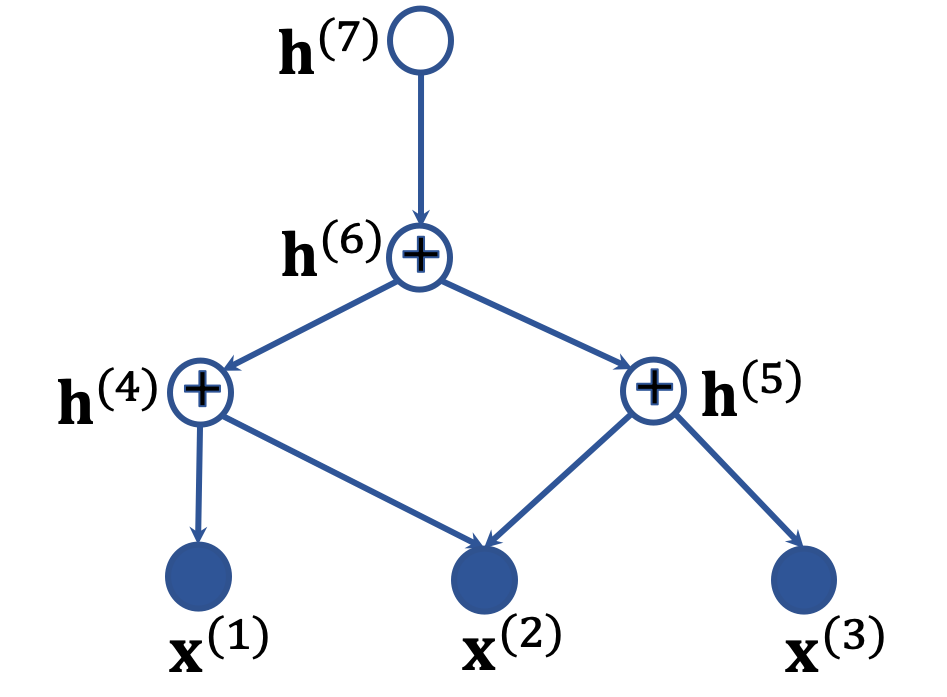
\includegraphics[width=2.3in]{fig/dag.png}
    \caption{DAG structure. The inverse topology order is \big\{ \{1,2,3\}, \{4,5\}, \{6\},  \{7\} \big\}, and it corresponds to layers 0 to 3.  }
    \label{fig:dag}
\end{figure}

Similarly the KL term can be expanded as in the tree structures. For nodes in layer $l$
\begin{align} \label{eq:KL_dag1}
-\textbf{\text{KL}}^{l:L} 
=&     \mathbb{E}_{q(\mathbf{h}^{pa(l)}|\mathbf{h}^l)} \big[ \log  p( \mathbf{h}^{l}|  \mathbf{h}^{pa(l)})    \big]  +  \textbf{\text{H}}(\mathbf{h}^{l}|\mathbf{h}^{ch(l)})  - \textbf{\text{KL}}^{l+1:L} \, .
\end{align}
The forward and backward messages or latent state of a node are stored in the message passing procedures. They can be used by the node's parents and children  to compute the ELBO.  
It enables the calculation even the parents or children are  not  in layer~$l+1$ or $l-1$. For the node $i$ in layer $l$,   $pa(i)$ may have children in layers below $l$. Some nodes in $l$ may not have parent, and combining with the prior, the entropy term will become an KL term in this case.  Thus,  we have 
\begin{align} \label{eq:KL_dag2}
-\textbf{\text{KL}}^{l:L} = &  \sum_{i:i\in l, i \not\in   \mathcal{R}_{ \mathcal{G}} }  \bigg\{ \mathbb{E}_{q(\mathbf{h}^{pa(i)}|\mathbf{h}^{ch(pa(i))}} \big[ \log p( \mathbf{h}^{i}|  \mathbf{h}^{pa(i)})    \big]   +  \textbf{\text{H}}_q(\mathbf{h}^{i}|\mathbf{h}^{ch(i)})  \bigg\}  \\ \notag
& -  \sum_{i \in l \bigcap \mathcal{R}_{ \mathcal{G} }  }  \textbf{\text{KL}}\big(q(\mathbf{h}^{(i)} | \mathbf{h}^{ch(i)} )   | p(\mathbf{h}^{(i)})  \big)  - \textbf{\text{KL}}^{l+1:L} \, .\notag
\end{align}

Recurrently applying~\eqref{eq:KL_dag2} yields
\begin{align} \label{eq:kl_dag3}
 \mathbb{E}_{q(\mathbf{h} | \mathbf{x})} \bigg[ \log  \frac{p( \mathbf{h})}{q(\mathbf{h}|\mathbf{x})}  \bigg] =& \sum_{l=1}^{L-1}   \sum_{i:i\in l, i \not\in   \mathcal{R}_{ \mathcal{G}}  }  \bigg\{ \mathbb{E}_{q(\mathbf{h}^{pa(i)}|\mathbf{h}^{(i)})} \bigg[ \log p( \mathbf{h}^{(i)}|  \mathbf{h}^{pa(i)})   \bigg]  +    \textbf{\text{H}}(\mathbf{h}^i | \mathbf{h}^{ch(i)} )  \bigg\} \\ \notag
& -   \sum_{l=1}^{L-1}  \sum_{i \in l \bigcap \mathcal{R}_{ \mathcal{G} }  }  \textbf{\text{KL}}\big(q(\mathbf{h}^{(i)} | \mathbf{h}^{ch(i)} )   | p(\mathbf{h}^{(i)})  \big)   -   \textbf{\text{KL}}\big(q(\mathbf{h}^L | \mathbf{h}^{L-1} )   | p(\mathbf{h}^L)  \big) \, .
 \end{align}
Since $L  \subseteq   \mathcal{R}_{ \mathcal{G}} $,  with $\mathbf{h}^{(0)} = \mathbf{x}$,~\eqref{eq:dag_elbo}, and~\eqref{eq:kl_dag3} we have 
\begin{align*}  
 \log p(\mathbf{x}) \geqslant  \mathcal{L}(\mathbf{x}; \theta) =&   \sum_{i \in \mathcal{G}  \setminus  \mathcal{R}_{ \mathcal{G} }  }  \mathbb{E}_{q(\mathbf{h}^{pa(i)}|\mathbf{h}^{ch(pa(i))})} \bigg[ \log p( \mathbf{h}^{(i)}|  \mathbf{h}^{pa(i)})   \bigg]  \\
 & +  \sum_{i \in \mathcal{G}  \setminus  \mathcal{R}_{ \mathcal{G} }  } \textbf{\text{H}}(\mathbf{h}^{(i)} | \mathbf{h}^{ch(i)} )   -    \sum_{i \in  \mathcal{R}_{ \mathcal{G} }  }  \textbf{\text{KL}}\big(q(\mathbf{h}^{(i)} | \mathbf{h}^{ch(i)} )   | p(\mathbf{h}^{(i)})  \big)  \, .
 \end{align*}


% \begin{figure*}[!htbp] %{r{0.4\textwidth}
% \begin{center}
%  %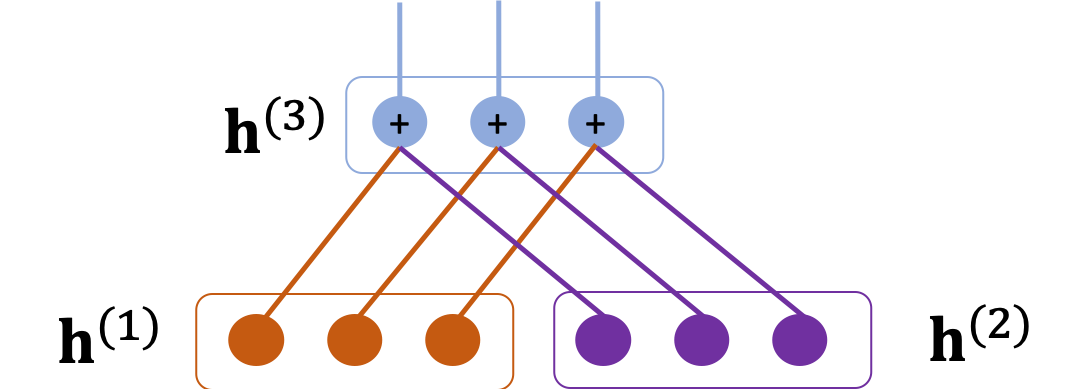
\includegraphics[width=0.43\linewidth]{fig/node_aggre_sum.png}
%  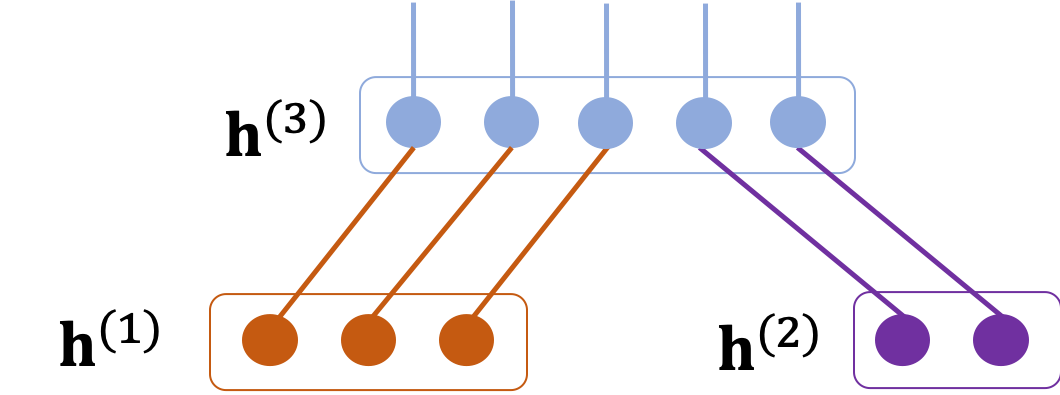
\includegraphics[width=0.43\linewidth]{fig/node_aggre_cat.png}
% \end{center}
%   \caption{Aggregation with concatenation.}
% \label{fig:node_aggre}
% \end{figure*}


\begin{figure*}[!htbp]%{r{0.4\textwidth}
\begin{center}
 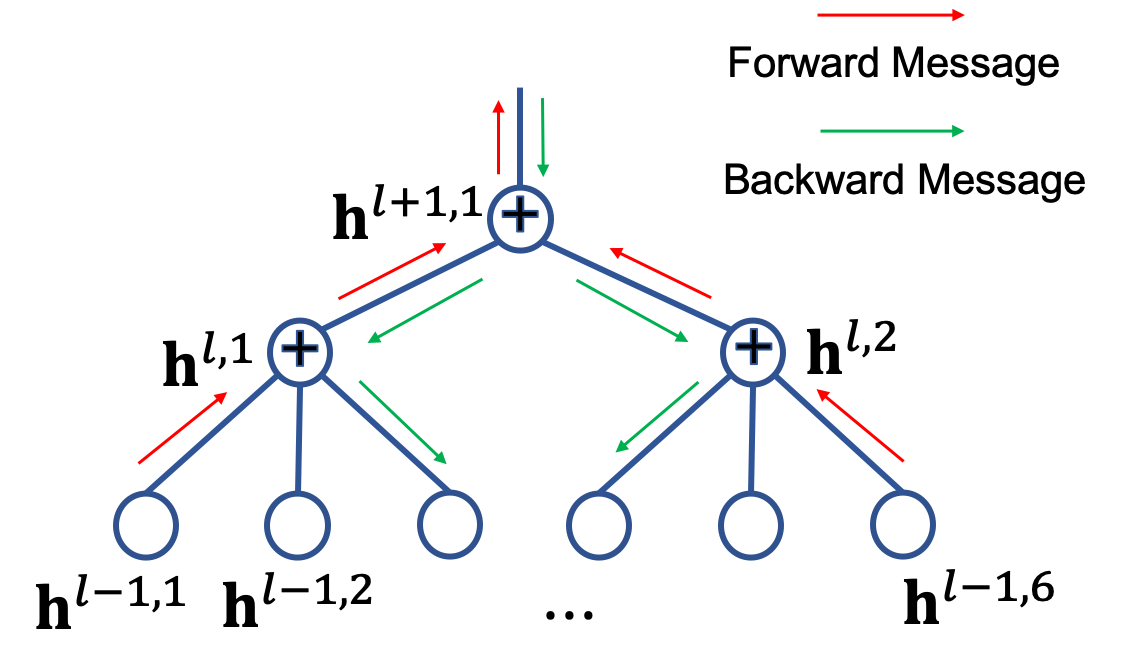
\includegraphics[width=0.5\linewidth]{fig/tree_message.png}
\end{center}
  \caption{Message passing on a tree.} 
\label{fig:message}
\end{figure*}

\section*{Appendix C.  Proof of Lemma1}\label{appd:proof_lm1}
\textbf{Lemma 1.} {\it Let $\mathcal{G}$ be a well trained tree structured variational flow graphical model with $L$ layers, and $i$ and $j$ are two leaf nodes with $a$ as the closest common ancestor. Given observed value at node $i$, the value of node $j$ can be approximated with   $\widehat{\mathbf{x}}^{j} \approx  \mathbf{f}_{(a,j)}(\mathbf{f}_{(i, a)}(\mathbf{x}^{(i)}))$. Here $\mathbf{f}_{(i, a)}$ is the flow function path from node $i$ to node $a$. The conditional density of $\mathbf{x}^{(j)}$ given $\mathbf{x}^{(i)}$ can be approximated with 
\begin{align*} %\label{eq:cond_llk}
\log p(\mathbf{x}^{(j)} | \mathbf{x}^{(i)}) &\approx  \log p(\widehat{\mathbf{h}}^L) -  \frac{1}{2} \log \big(\det \big(\mathbf{J}_{\widehat{\mathbf{x}}^{(j)}}(\widehat{\mathbf{h}}^L)^\top\mathbf{J}_{\widehat{\mathbf{x}}^{(j)}}(\widehat{\mathbf{h}}^L)\big) \big) \, .
\end{align*}
}
%\end{lemma}


\section*{Appendix D.  Proof of Theorem 1}\label{appd:proof_thm1}

\textbf{Theorem 1.} {\it Assume we observe data distributed according to the generative model given by~\eqref{eq:exp_h} and $\mathbf{x}^{(t)} = \mathbf{f}^{-1}_t(\mathbf{h}^{(t)}, \epsilon)$, we further have the following assumptions,

\vspace{0.05in}

(a) The sufficient statistics $T_{ij}(h)$ are differentiable almost everywhere and their derivatives $\frac{d T_{i,j}}{d h}$ are nonzero almost surely for all $h\in \mathcal{H}_i$ and all $1\leq i \leq d$ and $1 \leq j  \leq m$.

\vspace{0.05in}


(b) There exist $dm+1$ distinct conditions $\mathbf{u}^{(0)}$, ..., $\mathbf{u}^{(dm)}$  such that the matrix 
\begin{equation*} 
\mathbf{L} = [\mathbf{\lambda}(\mathbf{u}^{(1)}) - \mathbf{\lambda}(\mathbf{u}^{(0)}), ..., \mathbf{\lambda}(\mathbf{u}^{(dm)}) - \mathbf{\lambda}(\mathbf{u}^{(0)}) ]
\end{equation*} 
of size $dm \times dm$ is invertible.
Then the model parameters 
$\mathbf{T}(\mathbf{h}_k) = \mathbf{A}\widehat{\mathbf{T}}(\mathbf{h}_k) + \mathbf{c}.$ Here $\mathbf{A}$ is an $dm \times dm$ invertible matrix and $\mathbf{c}$ is a vector of size $dm$.
}

\begin{proof}
The conditional probabilities of $p_{\mathbf{T}, \mathbf{\lambda}, \mathbf{f}_t^{-1} }\big(\mathbf{x}^{(t)} | \mathbf{u}\big)$ and $p_{\widehat{\mathbf{T}}, \widehat{\mathbf{\lambda}}, \mathbf{g} }\big(\mathbf{x}^{(t)} | \mathbf{u}\big)$ are assumed to be the same in the limit of infinity data.  By expanding two pdfs with change of variable rule, we have 
\begin{align} \notag
\log p_{\mathbf{T}, \mathbf{\lambda}}(\mathbf{h}^{(t)}| \mathbf{u}) + \log \big| \det \mathbf{J}_{\mathbf{f}_t}(\mathbf{x}^{(t)}) \big| = \log p_{\widehat{\mathbf{T}}, \widehat{\mathbf{\lambda}}}((\mathbf{h}^{(t)})^\top| \mathbf{u}) + \log \big| \det \mathbf{J}_{g^{-1}}(\mathbf{x}^{(t)}) \big|.
\end{align}
 Let $\mathbf{u}^{(0)},...,\mathbf{u}^{(dm)}$ be from condition (b). We can subtract this expression for $\mathbf{u}^{(0)}$ for some condition $\mathbf{u}^{(v)}$. The Jacobian terms will be removed since they do not depend  $\mathbf{u}$,
\begin{align} \label{eq:u_diff}
\log p_{\mathbf{h}^{(t)}}(\mathbf{h}^{(t)}|\mathbf{u}^{(v)}) - \log p_{\mathbf{h}^{(t)}}(\mathbf{h}^{(t)}|\mathbf{u}^{(0)}) =\log p_{(\mathbf{h}^{(t)})^\top}((\mathbf{h}^{(t)})^\top|\mathbf{u}^{(v)}) - \log p_{(\mathbf{h}^{(t)})^\top}((\mathbf{h}^{(t)})^\top|\mathbf{u}^{(0)}).
\end{align}
Both conditional distributions of $\mathbf{h}^{(t)}$ given $\mathbf{u}$ belong to exponential family. Eq.~\eqref{eq:u_diff} can be rewritten as 
\begin{align} \notag
&\sum_{i=1}^l \bigg[\log \frac{Z_i(\mathbf{u}^{(0)})}{Z_i(\mathbf{u}^{(v)})} + \sum_{j=1}^m T_{i,j}(\mathbf{h}^{(t)})\big(\lambda_{i,j}(\mathbf{u}^{(v)})- \lambda_{i,j}(\mathbf{u}^{(0)})\big) \bigg] \\
= & \sum_{i=1}^l \bigg[\log \frac{\widehat{Z}_i(\mathbf{u}^{(0)})}{\widehat{Z}_i(\mathbf{u}^{(v)})} + \sum_{j=1}^m \widehat{T}_{i,j}(\mathbf{h}^{(t)})\big(\widehat{\lambda}_{i,j}(\mathbf{u}^{(v)})- \widehat{\lambda}_{i,j}(\mathbf{u}^{(0)})\big) \bigg].
\end{align}
Here the base measures $Q_i$ are cancelled out as they do not depend on $\mathbf{u}$. Let $\bar{\mathbf{\lambda}}(\mathbf{u}) = \mathbf{\lambda}(\mathbf{u})-\mathbf{\lambda}(\mathbf{u}^{(0)})$. The above equation can be rewritten with inner products as
\begin{align} \notag
\langle \mathbf{T}(\mathbf{h}^{(t)}), \bar{\mathbf{\lambda}}	\rangle + \sum_i \log \frac{Z_i(\mathbf{u}^{(0)})}{Z_i(\mathbf{u}^{(v)})}
=\langle \widehat{\mathbf{T}}((\mathbf{h}^{(t)})^\top), \widehat{\bar{\mathbf{\lambda}}}	\rangle + \sum_i\log \frac{\widehat{Z}_i(\mathbf{u}^{(0)})}{\widehat{Z}_i(\mathbf{u}^{(v)})}, \ \ \forall l, 1 \leq v \leq dm .
\end{align}
Combine $dm$ equations together and we can rewrite in matrix equation form as following
\begin{align} \notag
\mathbf{L}^{\top}\mathbf{T}(\mathbf{h}^{(t)}) = \widehat{\mathbf{L}}^{\top}\widehat{\mathbf{T}}((\mathbf{h}^{(t)})^\top) + \mathbf{b}.
\end{align}
Here $b_v=\sum_i\log \frac{\widehat{Z}_i(\mathbf{u}^{(0)}) Z_i(\mathbf{u}^{(v)}) }{\widehat{Z}_i(\mathbf{u}^{(v)}) Z_i(\mathbf{u}^{(0)}) }$. We can multiply $\mathbf{L}^{\top}$'s inverse with both sized of the equation, 
\begin{align}\label{eq:A_sim}
\mathbf{T}(\mathbf{h}^{(t)}) = \mathbf{A}\widehat{\mathbf{T}}((\mathbf{h}^{(t)})^\top) + \mathbf{c}.
\end{align}
Here $\mathbf{A} = \mathbf{L}^{-1\top} \widehat{\mathbf{L}}^{\top} $, and $\mathbf{c} = \mathbf{L}^{-1\top} \mathbf{b}$. 
By a lemma from~\cite{Khemakhem20a}, there exist $m$ distinct values $h^{(t,i)}_{1}$ to $h^{(t,i)}_{m}$ such that $\big[ \frac{d T_i}{ d h^{(t,i)}}(h^{(t,i)}_{1}), ...,  \frac{d T_i}{ d h^{(t,i)}}(h^{(t,i)}_{m}) \big]$ are linear independent in $\mathbb{R}^m$, for all $1\leq i \leq d$. Define $m$ vectors $\mathbf{h}^{(t)}_{v}= [h^{(t,1)}_v, ..., h^{(t,d)}_v]$ from points given by this lemma. We obtain the  Jacobian $\mathbf{Q}= [\mathbf{J}_{\mathbf{T}}(\mathbf{h}^{(t)}_1), ..., \mathbf{J}_{\mathbf{T}}(\mathbf{h}^{(t)}_m)]$ with each entry as Jacobian with size $dm \times d$ from the derivative of Eq.~\eqref{eq:A_sim} regarding these $m$ vectors. Hence $\mathbf{Q}$ is a $dm \times dm$ invertible by the lemma and the fact that each component of $\mathbf{T}$ is univariate. We can construct a corresponding matrix $\widehat{\mathbf{Q}}$ 
with the Jabocian $\widehat{\mathbf{T}}(\mathbf{g}^{-1}\circ \mathbf{f}_t^{-1}(\mathbf{h}^{(t)}))$ computed at the same points and get 
\begin{align} \notag
\mathbf{Q} = \mathbf{A}\widehat{\mathbf{Q}}.
\end{align}
Here $\widehat{\mathbf{Q}}$ and $\mathbf{A}$ are both full rank as $\mathbf{Q}$ is full rank.
\end{proof}


\end{document}